\documentclass[a4paper,fleqn]{cas-dc}
\usepackage[numbers]{natbib}
\usepackage[english]{babel}
\usepackage[utf8]{inputenc}
\usepackage[T1]{fontenc}
\usepackage{amsmath,amsfonts,amssymb,amsthm}
\usepackage{graphicx}
\usepackage{booktabs}
\usepackage{array}
\usepackage{tabularx}
\usepackage{longtable}
\usepackage{multirow}
\usepackage{float}
\usepackage{subcaption}
\usepackage[table,xcdraw,dvipsnames]{xcolor}
\usepackage{enumitem}
\setlist{noitemsep,topsep=3pt}

\usepackage{listings}
\lstset{basicstyle=\ttfamily\small, breaklines=true, frame=single, backgroundcolor=\color{gray!10}}
\usepackage{underscore}
\usepackage{siunitx}
\usepackage{tikz}
\usetikzlibrary{shapes.geometric,arrows}
\usepackage{pdflscape}
\usepackage{etoolbox}
\usepackage{makecell}

\numberwithin{equation}{section}
\numberwithin{figure}{section}
\numberwithin{table}{section}

\newcommand{\code}[1]{\texttt{#1}}

% Redefine paragraph so it is not run-in (add line break after title)
\makeatletter
\renewcommand\paragraph{\@startsection{paragraph}{4}{\z@}%
  {3.25ex \@plus1ex \@minus.2ex}%
  {0.5em}%
  {\normalfont\normalsize\bfseries}}
\newcommand{\subsubsubsection}[1]{\paragraph{#1}}
\makeatother

\let\WriteBookmarks\relax

% Float placement parameters
\renewcommand{\floatpagefraction}{0.85}   % min fraction of float page
\renewcommand{\textfraction}{0.05}        % min fraction of text in mixed page
\renewcommand{\topfraction}{0.92}         % max fraction for floats at top
\renewcommand{\bottomfraction}{0.5}       % max fraction for floats at bottom
\renewcommand{\dbltopfraction}{0.92}      % same, for two-column floats
\renewcommand{\dblfloatpagefraction}{0.85}
\setcounter{topnumber}{4}
\setcounter{bottomnumber}{2}
\setcounter{totalnumber}{6}
\setcounter{dbltopnumber}{4}

\begin{document}

\shorttitle{Forest carbon stock estimation in Spain}
\shortauthors{Gabriel-Vegas et al.}

\title [mode = title]{Data-driven estimation of forest carbon stocks in Spain: a machine learning approach using National Forest Inventory data}

\author[1]{Jaime Gabriel-Vegas}[type=editor]
\cormark[1]
\ead{JaimeGabrielVegas@usal.es}

\author[1]{Maider Araceli Urbón Jiménez}
\ead{murbon001@usal.es}

\author[1]{Ana de Luis Reboredo}
\ead{adeluis@usal.es}

\author[1]{Belén Pérez Lancho}
\ead{lancho@usal.es}

\author[1]{Ana-Belén Gil-González}
\ead{abg@usal.es}

\affiliation[1]{organization={Group B1, BISITE Research Team, University of Salamanca},
    addressline={Faculty of Sciences},
    city={Salamanca},
    country={Spain}}

\cortext[cor1]{Corresponding author}

\begin{abstract}
Forests are natural sinks of \(CO_2\) and their management is acquiring a central role in emission compensation regulatory frameworks and in voluntary carbon credit markets. However, the reliable estimation of the carbon that a forest plot will accumulate over a given time horizon remains a methodological challenge, especially when temporal projection from initial conditions is required. This work presents \textit{GreenWest}, a machine learning system to predict future forest carbon in Spain from stand structure, soil, climate and remote sensing data. Data come from the National Forest Inventory (IFN2 and IFN3), ERA5-Land climatic reanalysis, Landsat spectral indices and edaphic and topographic variables, integrated in a multi-source relational database. Through manual feature selection, an initial set of 445 predictors was reduced to 44 ecologically relevant variables, modelling two target variables: carbon density (\texttt{c4}, tC\,ha$^{-1}$) and total plot carbon (\texttt{carbono\_bruto4}, tC). \textit{Gradient boosting} models (LightGBM, XGBoost, CatBoost) and neural networks were trained and compared as base models, as well as stacking ensembles with different meta-model configurations. The best results are obtained with LightGBM and CatBoost ($R^2$ between 0.72 for IFN2/\texttt{c4} and 0.90 for IFN3/\texttt{carbono\_bruto4}), with systematic but modest improvements when incorporating stacking. Models trained on the combined IFN2$+$IFN3 set outperform local models on IFN2, while for IFN3 the opposite occurs. SHAP analysis reveals that tree density, species and canopy cover fraction are the dominant predictors, with the summer GNDVI index as the main spectral predictor; SHAP values are consistent with ecological knowledge, validating the model's capacity to learn relationships with genuine meaning.
\end{abstract}

\begin{keywords}
carbon credits \sep artificial intelligence \sep afforestation \sep reforestation \sep predictive modelling \sep climate change
\end{keywords}

\maketitle


% !TEX root = ../main_final_en.tex
\section{Introduction}

Climate change is one of the greatest global challenges and its most direct manifestation is the increase in atmospheric concentrations of carbon dioxide (\(CO_2\)), with impacts on the cryosphere, climate extremes and ecosystems \cite{IPCC2007}. Forests act as natural sinks by fixing \(CO_2\) in biomass via photosynthesis, making their management key for mitigation.


Over recent decades, international instruments such as the \textit{United Nations Framework Convention on Climate Change (UNFCCC)} and the \textit{Kyoto Protocol} \cite{UNFCCC1997,UNFCCC2015} have established regulatory frameworks for reducing greenhouse gas emissions through market-based mechanisms. In this context, \emph{carbon credits} arise: units representing the amount of carbon dioxide (\(CO_2\)), usually one tonne, that has been captured or whose emission has been avoided through certified mitigation projects.


Among eligible activities, afforestation and reforestation stand out for their capacity to act as natural carbon sinks, fixing \(CO_2\) in biomass and soil. However, for these actions to generate valid carbon credits they must meet a series of technical and legal criteria established in international climate change regulations and in their national application. In particular, these requirements derive from the forest sink accounting rules adopted under the United Nations Framework Convention on Climate Change (UNFCCC) and the Kyoto Protocol, as specified in the Marrakech Accords, as well as from the national forest definition communicated by Spain for these purposes \cite{UNFCCCMarrakech,UNFCCCSpainReview}. These criteria include:

\begin{itemize}
\item \textbf{Direct human intervention:}
The trees must result from direct human intervention activities such as planting, seeding or the deliberate promotion of natural regeneration. This requirement derives from the definition of \emph{afforestation} and \emph{reforestation} established in the Kyoto Protocol, which expressly excludes natural regeneration not induced by human action \cite{UNFCCCMarrakech}.

\item \textbf{Minimum permanence period:}
The project must ensure the permanence of the carbon sink for a prolonged period (usually on the order of 20--30 years), in order to guarantee that the captured carbon is not prematurely released into the atmosphere. This criterion responds to the permanence principle required in the LULUCF forest sink accounting regime and in national and European implementation frameworks, which excludes short-rotation crops whose carbon is released after harvest \cite{UNFCCCMarrakech,EULULUCF2018}.

\item \textbf{Minimum area of 1 hectare:}
The project area must have a minimum extent of 1 hectare. This threshold comes from Spain's national forest definition adopted within the ranges permitted by the Marrakech Accords (0.05--1 ha), officially communicated to the UNFCCC \cite{UNFCCCSpainReview}.

\item \textbf{Minimum canopy cover fraction of 20\%:}
For land to be considered forest, the crown cover of tree species must reach at least 20\% of the surface area. This value corresponds to Spain's national choice for the forest definition for climate accounting purposes \cite{UNFCCCSpainReview}.

\item \textbf{Minimum height of mature trees of 3 metres:}
Tree species must be capable of reaching a minimum height of 3 metres at maturity. It is not necessary for this height to be reached at the start of the project, but it must be attainable under normal growth conditions. This criterion is also part of Spain's national forest definition communicated in accordance with decisions adopted under the UNFCCC \cite{UNFCCCSpainReview}.
\end{itemize}

This work aims to obtain an artificial intelligence model to estimate the amount of carbon that a forest plantation in Spain will capture from vegetation, climate and terrain variables over a period of 20 to 30 years. This innovative approach has the potential to transform the management of afforestation and reforestation projects, optimising planting practices and maximising the amount of carbon that can be captured in these ecosystems.

The operational question is: \emph{given the initial characteristics of a plantation, how much \(CO_2\) will it contain after \(t\) years?, where \(t\) is a natural number.} To answer it, data from the \textbf{National Forest Inventory} (IFN2--IFN4, MITECO) \cite{ifn}, \textbf{ERA5-Land} reanalysis \cite{era5land} and \textbf{Landsat spectral indices} (Collection~2, L2) \cite{landsatc2} are integrated into a hierarchical relational database described in a companion work \cite{greenwestdb}.

This model will not only improve understanding of the behaviour of carbon sinks, but will also provide useful tools for strategic decision-making in both business and environmental spheres. In this way, the \textit{GreenWest} project contributes to the transition towards a low-carbon economy, aligning with the global sustainability objectives established within the framework of the UNFCCC and the \textit{Kyoto Protocol}, and promoting the creation of a more efficient and accessible carbon credit market for the economic actors involved in the management of natural resources.



% !TEX root = ../main_final_en.tex
\section{Objectives and Justification}

The main objective of this study is to develop an artificial intelligence model capable of accurately predicting the capacity of Spanish forest plantations to absorb carbon dioxide (\(CO_2\)). This model is based on variables describing tree species, terrain characteristics and climatic and meteorological conditions. From this general objective, several specific goals are derived, which together justify the relevance and applicability of the project.

\subsection{Specific objectives}

The main objectives are listed below:

\begin{itemize}
    \item \textbf{Develop a robust predictive model:} Build a machine learning model that estimates the amount of \(CO_2\) that will be captured over time by a forest plantation, based on data such as species, soil type, diameter class, climate and other relevant variables.

    % \item \textbf{Optimise carbon capture:} Use the model to identify optimal combinations of species and terrain that maximise carbon fixation, contributing to the efficient planning of (re)forestation projects.

    \item \textbf{Ensure compliance with international regulations:} Guarantee that the model's predictions and outputs are compatible with the regulatory frameworks defined by the \textit{United Nations Framework Convention on Climate Change} (UNFCCC) and the \textit{Kyoto Protocol}, thus meeting the criteria required for the validation of carbon credits.

    \item \textbf{Analyse the determining factors of forest development:} Study the influence of climatic variables (such as temperature and precipitation) and edaphic variables (such as soil type or slope) on forest growth and its carbon capture capacity.

    \item \textbf{Support environmental and business decision-making:} Provide a practical and validated tool that enables technicians, managers and companies to select the most suitable species and plan afforestation actions with maximum efficiency in terms of carbon sequestration.
\end{itemize}

\subsection{Justification}

The need for predictive tools to estimate \(CO_2\) capture has intensified given the growth of the voluntary carbon credit market, and the obligations acquired: each country must report its greenhouse gas emissions and absorptions, and can use (re)forestation activities as offsetting mechanisms.

For these projects to be eligible, they must meet specific criteria, which make it essential to have models that not only estimate current carbon but are capable of forecasting its future evolution based on initial conditions and predictor variables.

This work seeks to fill that gap through the use of artificial intelligence applied to real, multi-source data. Integrating its management within the carbon credit system can represent an important opportunity for the local economy, which could support those regions where depopulation and the demographic challenge are a serious problem, and for the mitigation of climate change.



% !TEX root = ../main_final_en.tex
% sections/03_literature_review.tex
\section{Literature Review}

The precise quantification of forest resources has historically been one of the cornerstones of territorial management and natural resource economics. The evolution of techniques for measuring tree growth and, more recently, for estimating biomass and carbon content, reflects a profound transformation in human society's priorities with respect to forest ecosystems. What began in medieval Europe as a logistical need to ensure the supply of firewood and structural timber in the face of scarcity has metamorphosed in the 21st century into a high-technology scientific discipline driven by global climate urgency \cite{brack_history_2000}.

Traditional dendrometry, the pillar of modern forest inventories, is based on the use of allometric relationships to estimate biomass ($w$) and other ecological parameters from easily measurable field variables, mainly diameter at breast height ($D$) and total height ($H$). These estimates are usually articulated through equations of the form:
\begin{equation}
    w = a D^b H^c
\end{equation}
or their logarithmic transformations:
\begin{equation}
    \lg w = a + b \lg D + c \lg H
\end{equation}
where parameters $a, b$ and $c$ are empirical regression coefficients \cite{shi2017methods}. In this context, the precision of primary measurements is critical, since, given the potential nature of these functions, errors in measuring $D$ and $H$ propagate and amplify in the final calculation of volume and carbon content. Despite the apparent simplicity of the fitting, results can be very good, as shown in Figure~\ref{fig:moso_bamboo}. However, there is a tension in the literature between the use of ``pantropical'' or generalised equations and species- or site-specific equations, since biases can be introduced if the architecture of local trees differs from the global one \cite{shang2025allometric}.

\begin{figure}
    \centering
    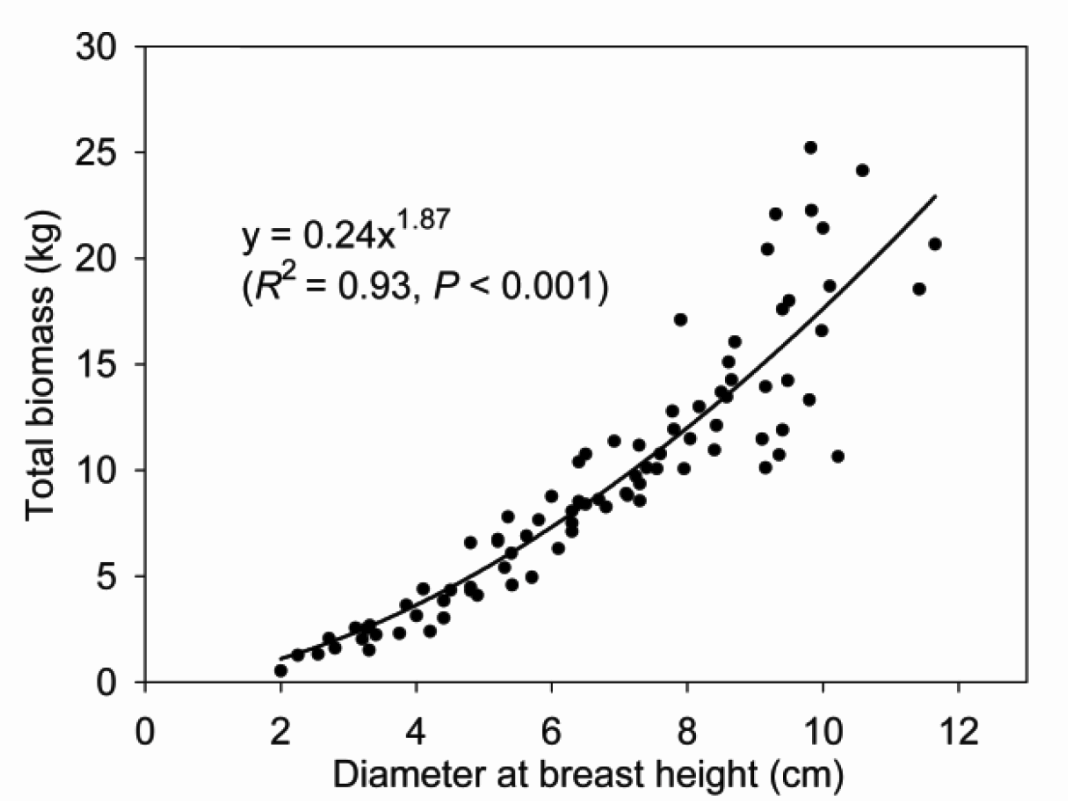
\includegraphics[width=\linewidth]{figuras/03_revision_literatura/moso_bamboo.png}
    \caption{Relationship between total biomass in kilograms and diameter at breast height in centimetres for moso bamboo \textit{(Phyllostachys edulis)}. Seen in \cite{shi2017methods}, with \cite{qi2016combining} as the original source.}
    \label{fig:moso_bamboo}
\end{figure}



The measurement of tree height has historically posed a greater challenge than that of diameter. Until the 1990s, mechanical hypsometers based on trigonometry predominated, which required manually measuring the distance to the tree and a clear line of sight \cite{nyakudanga_treemes}. These methods suffered from limitations of accuracy and ergonomics. The introduction of electronics marked a turning point by using ultrasound to measure distances automatically, enabling work in dense understoreys and improving precision to below 1\% \cite{nyakudanga_treemes}. At the same time, modern electronic callipers (an instrument measuring the linear distance between two parallel tangents to the tree stem) have digitised data collection, integrating measurement and metadata recording to minimise transcription errors \cite{nyakudanga_treemes}.

Subsequently, the introduction of laser scanning technology represented a revolution in forest measurement, overcoming the logistical and accuracy limitations of traditional methods. This technology is deployed mainly in two modalities: terrestrial laser scanning (TLS), which captures the three-dimensional structure of the forest from the ground with millimetre detail \cite{Kristiansen2018}, and airborne LiDAR. The latter is a method that uses light pulses to measure distances. Large-scale surveys typically consist of a LiDAR system mounted on an aircraft, helicopter, drone or satellite, which measures the distance to objects below it. One advantage is that, just as light can reach the ground through gaps in tree crowns, LiDAR laser pulses do so too, as we can observe in Figure~\ref{fig:lidar_avion}.
\begin{figure}
    \centering
    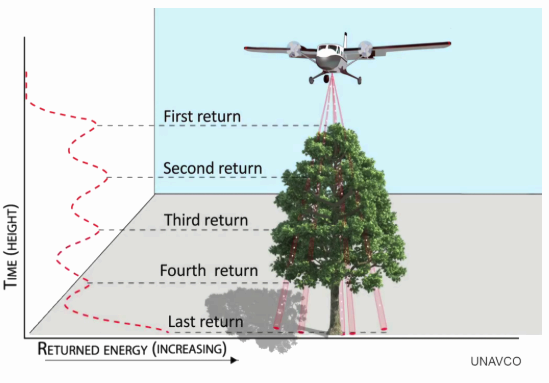
\includegraphics[width=\linewidth]{figuras/03_revision_literatura/lidar_avion.png}
    \caption{Diagram of a tree being scanned by an airborne LiDAR system and the various reflected pulses. Image obtained from \cite{opentopography_lidar_basics}.}
    \label{fig:lidar_avion}
\end{figure}
This means that in a single overflight various layers at different heights can be captured, enabling 3D reconstructions of the scanned area. The level of detail achievable is so high that individual trees can be identified, as seen in Figure~\ref{fig:chm_example}.


\begin{figure}
    \centering
    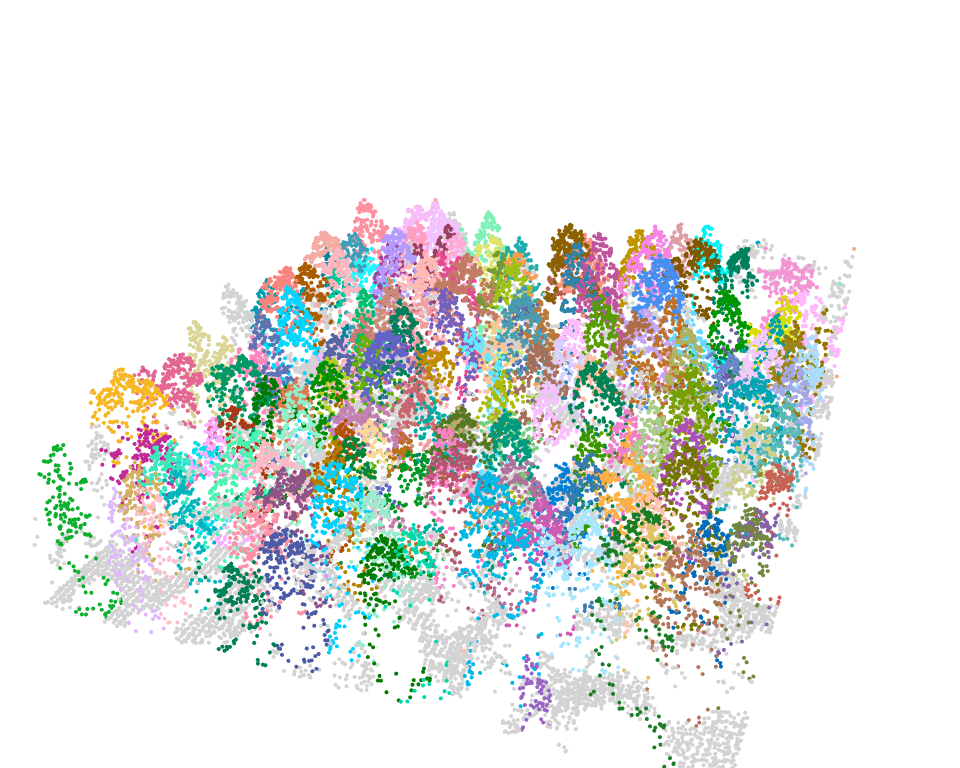
\includegraphics[width=\linewidth]{figuras/03_revision_literatura/CHM_1.png}
    \caption{Visualisation of a forest scanned with LiDAR. The possibilities of identifying individual trees in a dense forest environment are shown \cite{roussel2024lidrbook_itd}.}
    \label{fig:chm_example}
\end{figure}


% \begin{figure}
%     \centering
%     \begin{subfigure}[b]{0.48\linewidth}
%     \centering
%     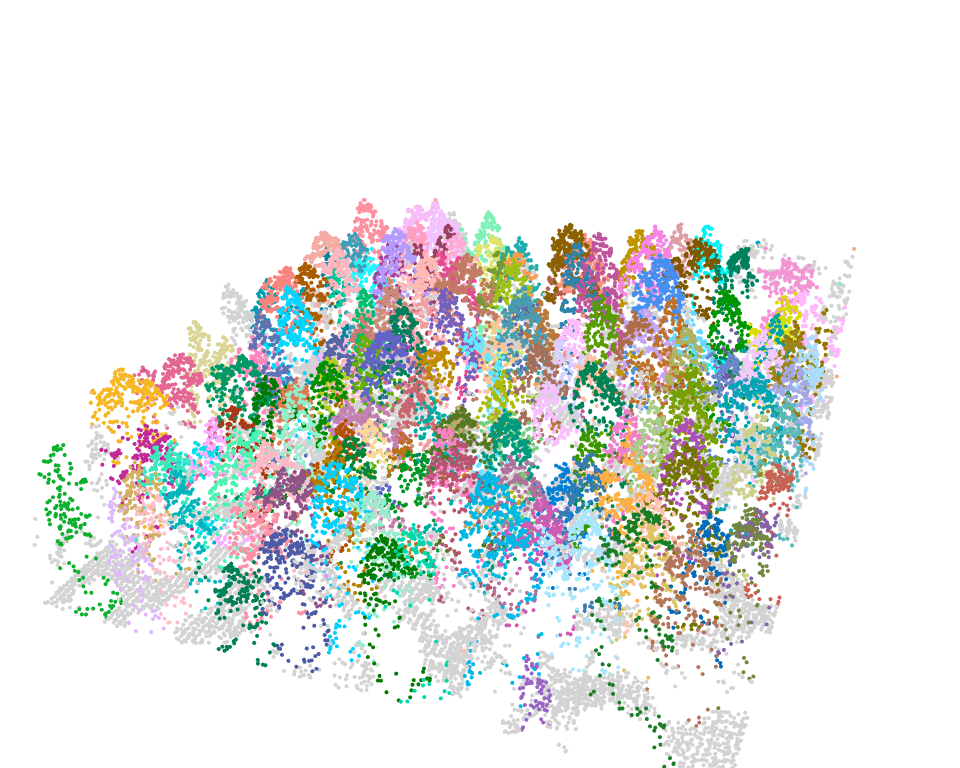
\includegraphics[width=\linewidth]{figuras/03_revision_literatura/CHM_1.png}
%     \caption{3D visualisation of a forest scanned with LiDAR. Each tree has been identified with a different colour.}
%     \label{fig:lit_sub1}
%     \end{subfigure}
%     \hfill
%     \begin{subfigure}[b]{0.48\linewidth}
%         \centering
%         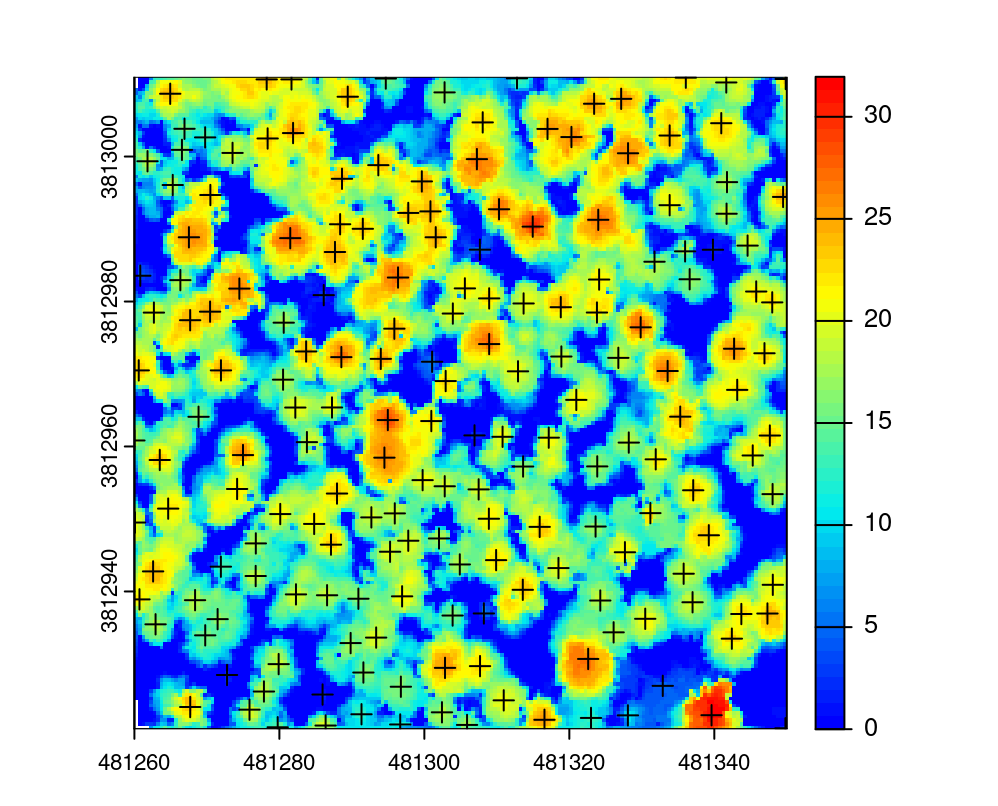
\includegraphics[width=\linewidth]{figuras/03_revision_literatura/CHM_2.png}
%         \caption{Same mapping but seen from above as a 2D map. Each tree is marked with an \textbf{x}.}
%         \label{fig:lit_sub2}
%     \end{subfigure}
%     \caption{Visualisation of a forest scanned with LiDAR. The possibilities of identifying individual trees in a dense forest environment are shown.}
%     \label{fig:chm_example}
% \end{figure}

The main limitations of airborne LiDAR lie in its high cost and logistical complexity. These factors hinder large-scale coverage with optimal periodicity, also generating significant latency in the availability of regional data. Furthermore, processing this information is more demanding than previous methods, compounded by the technical challenge of managing and storing large volumes of data. Figure~\ref{fig:pnoa_lidar} shows the data acquisition plan for the Third cycle of the PNOA-LiDAR project of Spain's National Geographic Institute, where the cadence of mappings can be appreciated.

\begin{figure}
    \centering
    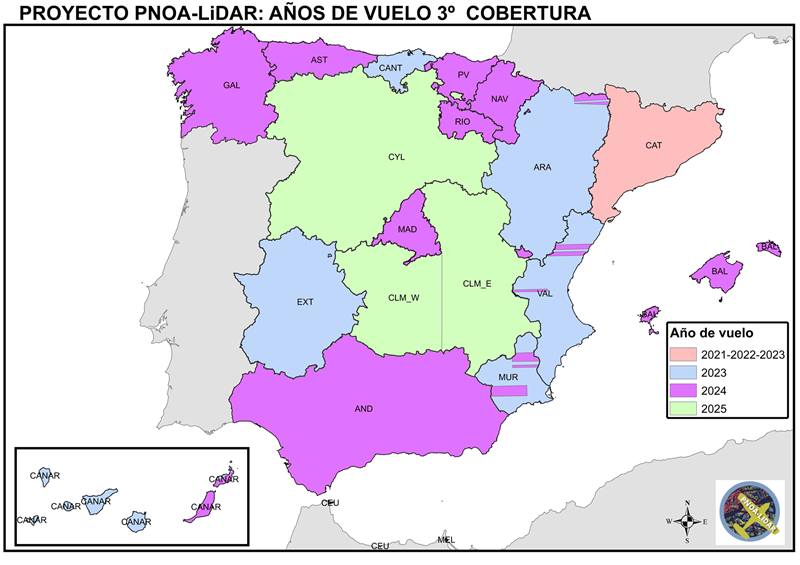
\includegraphics[width=\linewidth]{figuras/03_revision_literatura/plan_lidar_mapeo.png}
    \caption{Data acquisition plan for the Third cycle of the PNOA-LiDAR project of Spain's National Geographic Institute \cite{ign_pnoa_lidar_tercera}.}
    \label{fig:pnoa_lidar}
\end{figure}


The integration of these structural data, together with satellite remote sensing and the large-volume data processing capability offered by machine learning algorithms, has inaugurated a new paradigm: the ability to monitor forest resources at global scale with unprecedented precision. It is in this context of ``precision forestry'' and large-scale Earth observation that current research is situated, with very promising results having been achieved that enable the complexity of forest ecosystems to be addressed with a granularity previously unattainable.



% !TEX root = ../main_final_en.tex
\section{State of the Art}
\label{sec:estado-del-arte}

Carbon sequestration in forest ecosystems has gained growing importance in the scientific literature, driven both by international commitments on climate change and by the rise of carbon credit markets. This has motivated the development of models aimed at quantifying forest biomass and estimating carbon content, taking advantage of recent advances in remote sensors and artificial intelligence techniques.


One of the most established strategies for quantifying forest carbon is the estimation of stored carbon at a given moment from remote sensing data. Goetz et al. (2009) \cite{goetz2009remote} review the use of satellite observations, including optical sensors such as MODIS and Landsat, in empirical models of aboveground biomass, highlighting their applicability at regional scale, especially in boreal ecosystems. These types of estimates are usually based on linear regressions or generalised least squares models, with coefficients of determination typically between 0.6 and 0.8, depending on spatial resolution and ecosystem heterogeneity.

The application of deep learning has substantially improved the accuracy and spatial resolution of these estimates. For example, Zhang et al. (2022) \cite{zhang2022carbon} integrate Sentinel-2 imagery with convolutional neural networks, achieving an \(R^2\) of 0.84 for estimating carbon in subtropical forests. Similarly, Jiang et al. (2022) \cite{jiang2022integrating} develop the \textit{ForestCarbonAI} model, trained with multispectral and LiDAR data, generating high-resolution (10~m) forest carbon maps and reporting mean absolute errors (MAE) below 3.5 tC/ha in temperate zones. Other recent works, such as Reiersen et al. (2022) \cite{reiersen2022reforestree} or Dong et al. (2023) \cite{dong2023forest}, also demonstrate the effectiveness of \textit{deep learning} for static estimates, although they focus on tropical contexts and do not consider the temporal component.


In contrast to these descriptive approaches, some initiatives have attempted to project the evolution of carbon into the future. At the national level, the Ministry for Ecological Transition (MITECO) has implemented tools such as the \textit{ex ante} carbon absorption calculator \cite{miteco_abexante_2025}, which provides simplified estimates of the carbon that can be fixed in a forest plantation depending on species and agroclimatic zone. However, this instrument is based on tabulated coefficients and does not incorporate real edaphoclimatic variables or data-based modelling techniques, which limits its accuracy and ability to adapt to specific contexts.

At the European level, the work of Fasihi et al. (2024) \cite{fasihi2024assessing} stands out, applying an approach similar to that proposed in this study in the Friuli-Venezia Giulia region (Italy). Their objective is to estimate both the current carbon \textit{stock} and its annual absorption rate (sequestration), based on dendrochronology data from the Italian National Forest Inventory. These measurements, carried out between 2017 and 2019, quantify the radial growth of the last five years to estimate biomass through allometric equations and its conversion to carbon according to IPCC guidelines. They then train predictive models using meteorological, geomorphological variables, vegetation indices and a LiDAR canopy height model (CHM), attempting to predict the values obtained from field data.

The authors evaluate various ensemble models, reporting that combinations of algorithms such as Random Forest, AdaBoost and CatBoost offer the best performance. In predicting carbon \textit{stock}, they achieve an $R^2$ of $0.73 \pm 0.07$ and an RMSE of $31.55 \pm 9.35$ tC/ha. For the sequestration rate, results are more modest, with an $R^2$ of $0.42 \pm 0.08$ and an RMSE of $0.90 \pm 0.08$ tC/ha/year. A key finding of the study is that the inclusion of LiDAR data dramatically improves the accuracy of estimates.




In this scenario, the present work proposes an innovative methodology focused on dynamic long-term carbon prediction. Unlike previous models, which estimate already-stored carbon, this study focuses on anticipating how much carbon a forest plantation will capture over a specific time horizon. To this end, various supervised learning models are studied, trained with historical data from the National Forest Inventory (IFN2, IFN3 and IFN4) \cite{ifn} including edaphic characteristics, climatic variables from Copernicus \cite{copernicus_temps,copernicus_pr} and spectral metrics derived from Landsat images \cite{landsat5_data}. Details on the model architecture, variables used, algorithms implemented and evaluation metrics are developed in the following sections.





% !TEX root = ../main_final_en.tex
\section{Methodology}

This section describes the procedure followed for training and validating the predictive models. The methodology is grounded in the factors that determine forest growth: meteorological conditions (temperature, precipitation) affect photosynthesis and water availability; aspect, slope and altitude modulate incident radiation and local microclimate; and tree density determines intraspecific competition \cite{IPCC2006}. The approach integrates structural, climatic and spectral information from the IFN and complementary environmental sources to predict carbon accumulated in living biomass.


\subsection{Data origin and structure}

The database integrates forest, climatic and spectral information at the plot, species and diameter class level, structured around the IFN2, IFN3 and IFN4 inventories. In addition to the IFN dendrometric variables, each plot incorporates seasonal climatic statistics (temperature, precipitation, Martonne index) and spectral indices derived from satellite imagery (NDVI, EVI, NDII, GNDVI). Figure~\ref{fig:GWestBBDD} shows the relational schema of the main tables; a complete variable dictionary is given in \cite{greenwestdb}.

\begin{figure}
    \centering
    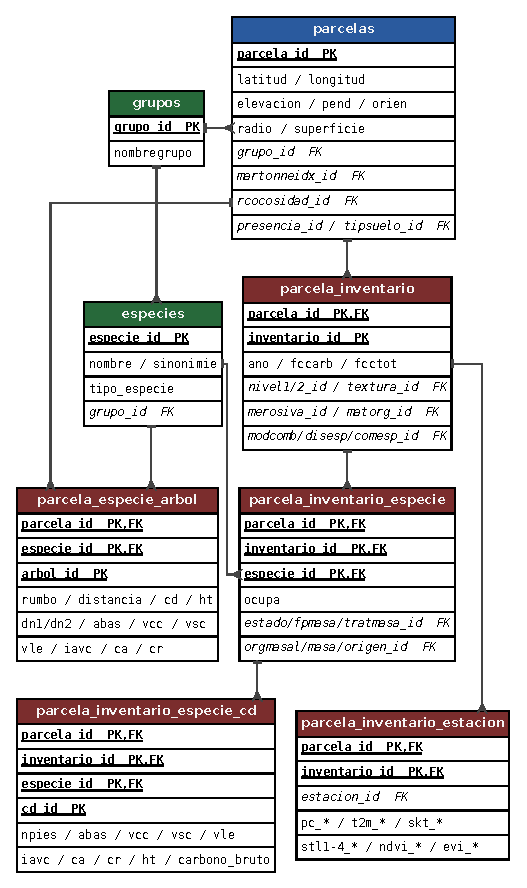
\includegraphics[width=\linewidth]{figuras/05_metodologia/er_diagram.pdf}
    \caption{Relational schema of the main database tables. Figure extracted from \cite{greenwestdb}, where further details on the variables can be found.}
    \label{fig:GWestBBDD}
\end{figure}


\subsection{Target variables}

The goal of the model is to estimate the \textbf{total carbon} that a forest plot will capture over a time horizon of 20--30 years, based on conditions observed in previous inventories.
Two complementary response variables are considered, both derived from the National Forest Inventory (IFN) data, allowing carbon content to be analysed from different perspectives: one normalised by area and another in absolute terms.


\begin{enumerate}
    \item \textbf{\texttt{c}} (tC/ha): represents the \textbf{total carbon contained in aboveground and belowground living biomass} per unit area, expressed in \emph{tonnes of carbon per hectare}.
          Its calculation is based on the sum of the aboveground (\texttt{ca}) and root (\texttt{cr}) carbon estimates reported by the IFN.
          In cases with missing values, the information was completed using a \emph{Random Forest Regressor} model fitted on observed dendrometric variables (Species, CD, VSC, NPies, ABas, IAVC, VCC and VLE), achieving satisfactory performance (\(R^2_{test} > 0.90\)).
          This variable is consistent with international forest inventory reporting formats and allows carbon content to be compared across plots or species.


    \item \textbf{\texttt{carbono\_bruto}} (tC): corresponds to the \textbf{total carbon captured per plot and species}, expressed in \emph{total tonnes of carbon}.
          Its estimation is performed in a traceable and physically interpretable manner from variables measured directly in the field: number of trees (\texttt{npies}), mean height (\texttt{ht}), species type (\texttt{clase\_especie}) and diameter class (\texttt{cd\_id}).
          The calculation follows an allometric model adapted from \cite{chave2014} and the IPCC guidelines~\cite{IPCC2006}, incorporating both aboveground and root biomass via the Root-to-Shoot ratio ($R$).
          The result is expressed in total tonnes of carbon per plot, without normalisation by area, which facilitates the traceability of the process and the comparison between inventories without depending on IFN-specific expansion factors.
          Consistent with the criteria for afforestation and reforestation projects, observations corresponding to seedlings or saplings are assigned a zero carbon value, since early development stages are not officially counted as captured carbon.
\end{enumerate}


These two variables summarise forest carbon content from complementary perspectives:
\texttt{c} (tC/ha) enables spatial and temporal comparison between forest stands, while \texttt{carbono\_bruto} (tC) provides an absolute measure directly derived from field observations.
Both constitute the main targets of the predictive modelling, aimed at estimating the carbon accumulated in \textbf{IFN4} from the conditions recorded in the previous inventories (\textbf{IFN2} and \textbf{IFN3}).

For further details on the origin of these variables, see \cite{greenwestdb}.

\subsection{Eligibility assumptions and external verification}
% Intervención humana, permanencia 30a (extrapolación cauta), superficie>=1ha,
% fccarb>=20% (filtro), altura>=3m en madurez (decisión de diseño).
As already introduced, for a forest project to be eligible for \emph{carbon credit} programmes in Spain, certain technical requirements must be met \cite{IPCC2006, miteco_guia_co2}. Each criterion and the way it is addressed in this study are summarised below:

\begin{itemize}
    \item \textbf{Direct human intervention.} The carbon increment must result from planned actions (reforestation, restoration or sustainable management). In our case, the model is trained on observational data (IFN2--IFN3--IFN4); therefore, \emph{intervention verification} is not inferred from the model, but is considered as an \emph{external condition} of eligibility for the project to be evaluated.

    \item \textbf{Minimum permanence.} The interval between IFN3 and IFN4 is mostly between 6 and 17 years (Figure~\ref{fig:periodo34}), a range too narrow for the 20--30 year reference horizon. To extend temporal coverage, the IFN2--IFN3 pair was also integrated, yielding intervals of 6 to 29 years (Figure~\ref{fig:periodo234}), more representative of the target horizon.

          \begin{figure}
              \centering
              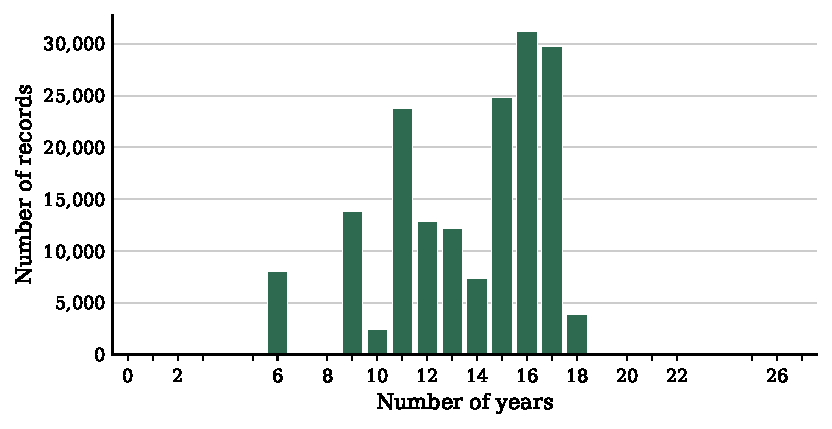
\includegraphics[width=\linewidth]{figuras/05_metodologia/hist_periodo_ifn34.pdf}
              \caption{Distribution of the year difference between the third and fourth inventories.}
              \label{fig:periodo34}
          \end{figure}

          \begin{figure}
              \centering
              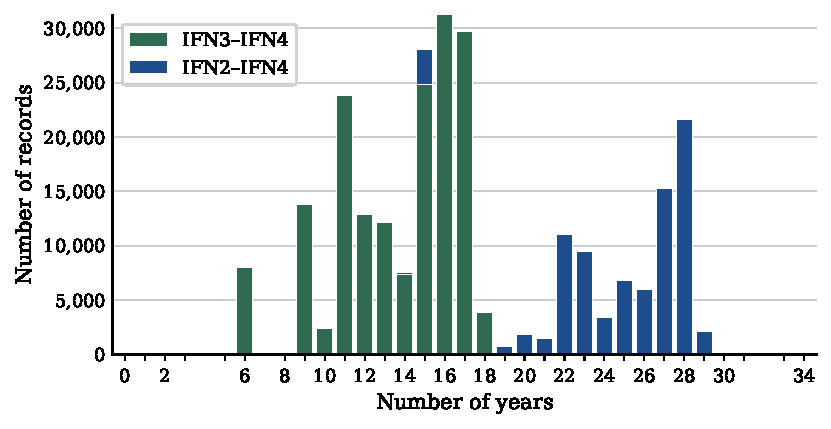
\includegraphics[width=\linewidth]{figuras/05_metodologia/hist_periodo.pdf}
              \caption{Distribution of the year difference between the IFN2--IFN3 and IFN3--IFN4 inventories.}
              \label{fig:periodo234}
          \end{figure}

    \item \textbf{Minimum area of 1 ha.} This is a criterion external to the model, verifiable \emph{ex ante} from the declared project geometry. In homogeneous stands, total carbon is approximately proportional to area, so this requirement does not affect model fitting.

    \item \textbf{Minimum canopy cover fraction of 20\%.} The database provides \texttt{fccarb} (tree canopy cover) and \texttt{fcctot} (total cover). This threshold is applied as an \emph{eligibility filter} prior to modelling ($\texttt{fccarb} \geq 20$).

    \item \textbf{Minimum height of 3 m at maturity.} This refers to the adult height of the species, not to the seedlings at the time of inventory. It is evaluated externally through the selection of appropriate species and does not intervene in model training.
\end{itemize}

\subsection{Data preparation and processing}
% Filtros (fccarb>=20%, crecimiento positivo, etc.)
% Agregaciones (parcela-especie, compresión CD -> npies_{cd}, etc.)
% Cálculo de variables derivadas (carbono\_bruto)
% Codificación y escalado

As already introduced, training is carried out along two lines according to the target variable: carbon in tonnes per hectare (\texttt{c} from \textbf{IFN4}) or carbon in tonnes (\texttt{carbono\_bruto} from \textbf{IFN4}); and according to the information used as explanatory variables: \textbf{IFN3} or \textbf{IFN3} and \textbf{IFN2}. Data preparation and filtering are presented in general terms.

\subsubsection{Record filtering}\label{subsec:filtradoregistros}

All plots in which the total carbon value (target variable) at the second inventory is lower than at the first are discarded. These cases are usually due to deforestation episodes, fires or other disturbances, and do not represent net forest growth.


The dataset is restricted to plots with a \texttt{fccarb} (tree canopy cover fraction) equal to or greater than 20\,\% in the explanatory inventory. This threshold defines the minimum proportion of area occupied by tree crowns relative to the total plot area, and constitutes one of the essential conditions for considering a surface as forest land. Excluding plots with \texttt{fccarb} below 20\,\% ensures that carbon estimates are made on consolidated forest stands, avoiding biases associated with agricultural areas or shrublands. The \textbf{IFN2} data are not subject to this filter because the \texttt{fccarb} variable is not available for that inventory.


\subsubsection{Variable calculation and aggregation}

Each input record is generated at the plot--species combination level, incorporating the corresponding variables from the first measurement and the target variable (carbon) from the second measurement (IFN4). The \texttt{parcela} and \texttt{parcela\_inventario} variables are split for each species. The entries in the \texttt{parcela\_inventario\_especie\_cd} table are grouped by plot and species and compressed into a single entry by creating a set of variables for each diameter class.


% La Tabla~\ref{tab:entradamodelo} resume las variables empleadas como entrada al modelo, integradas desde las distintas tablas que conforman la base de datos relacional.

% \begin{table*}
%     \renewcommand{\arraystretch}{1.2}
%     \setlength{\tabcolsep}{3pt}
%     \centering
%     \footnotesize
%     \resizebox{\textwidth}{!}{
%         \begin{tabular}{|p{3.2cm}|p{1.8cm}|p{6.5cm}|p{2.2cm}|}
%             \hline
%             \multicolumn{4}{|c|}{\textbf{Model Input Data Summary}}                                                                                                                                                                                                                                                                  \\
%             \hline
%             \textbf{Variable}                                                                                                                                                                 & \textbf{Type} & \textbf{Description}                              & \textbf{Annex}                                                                 \\
%             \hline
%             \textcolor{ForestGreen}{\texttt{parcela\_id}}                                                                                                                                     & varchar       & Unique plot identifier.                   & --                                                                             \\
%             \hline
%             \textcolor{ForestGreen}{\texttt{especie\_id}, \texttt{tipo\_especie}, \texttt{grupo\_id}}                                                                                         & int (CF)      & Species, type and taxonomic group.                 & \ref{sec:especies}, \ref{sec:gruposespecies}                                   \\
%             \hline
%             \textcolor{ForestGreen}{\texttt{ocupa}}                                                                                                                                           & int           & Occupancy degree (0--10).                       & --                                                                             \\
%             \hline
%             \textcolor{ForestGreen}{\texttt{estado\_id}}, \texttt{fpmasa\_id}, \texttt{tratmasa\_id}, \texttt{orgmasa1\_id}                                                                   & int (CF)      & State, stand form, treatment, organisation. & \ref{sec:EstadoIFN34}, \ref{sec:FPMasa}, \ref{sec:tratmasa}, \ref{sec:OrgMasa} \\
%             \hline
%             \textcolor{ForestGreen}{\texttt{tipsuelo1-3\_id}}                                                                                                                                 & int (CF)      & Soil types.                                   & Annex \ref{sec:TipSuelo}                                                       \\
%             \hline
%             \textcolor{ForestGreen}{\texttt{rocosidad\_id}}, \texttt{textura\_id}, \texttt{matorg\_id}, \texttt{modcomb\_id}, \texttt{disesp\_id}, \texttt{comesp\_id}, \texttt{merosiva\_id} & int (CF)      & Edaphic and structural variables.               & Various appendices                                                               \\
%             \hline
%             \textcolor{ForestGreen}{\texttt{radio}, \texttt{orientacion}, \texttt{elevacion}, \texttt{pendiente}}                                                                             & float         & Topography and plot geometry.                & --                                                                             \\
%             \hline
%             \textcolor{ForestGreen}{\texttt{martonneidx\_id}}                                                                                                                                 & int (CF)      & Martonne aridity index.                     & --                                                                             \\
%             \hline
%             \texttt{nivel1\_id}, \texttt{nivel2\_id}, \texttt{fccarb}, \texttt{fcctot}                                                                                                        & int/float     & Hierarchical levels and canopy cover.            & \ref{sec:nivel1}, \ref{sec:nivel2}                                             \\
%             \hline
%             \textcolor{ForestGreen}{\texttt{npies\_\{CD\}}}                                                                                                                                   & float         & Number of trees per diameter class.                 & --                                                                             \\
%             \hline
%             \textcolor{ForestGreen}{\texttt{periodo}}                                                                                                                                         & int           & Years between inventories.                           & --                                                                             \\
%             \hline
%             \textcolor{ForestGreen}{\texttt{evi, gndvi, ndii, ndvi\_\{stat\}\_\{est\}}}                                                                                                       & float         & Vegetation indices by season.               & --                                                                             \\
%             \hline
%             \textcolor{ForestGreen}{\texttt{pr, skt, stl1-4, t2m\_\{stat\}\_\{est\}}}                                                                                                        & float         & Climatic variables by season.                & --                                                                             \\
%             \hline
%             \textcolor{ForestGreen}{\texttt{c4}, \texttt{carbono\_bruto4}}                                                                                                                    & float         & IFN4 carbon (t/ha and t).                          & --                                                                             \\
%             \hline
%         \end{tabular}
%     }
%     \caption{Model input variables. Variables in \textcolor{ForestGreen}{green} are available in IFN2 and IFN3; the rest only in IFN3.}
%     \label{tab:entradamodelo}
% \end{table*}


\subsubsection{Reclassification of the \texttt{pendiente} and \texttt{orientacion} variables}

Since the ecological effect of slope and aspect on carbon accumulation is non-linear, both variables were reclassified as categorical factors. The \texttt{pendiente\_cat} variable was defined using seven intervals ($<5^\circ$, $5$--$10^\circ$, $10$--$15^\circ$, $15$--$20^\circ$, $20$--$30^\circ$, $30$--$50^\circ$, $>50^\circ$); the \texttt{orientacion\_cat} variable into eight equiangular cardinal sectors (\texttt{N}, \texttt{NE}, \texttt{E}, \texttt{SE}, \texttt{S}, \texttt{SO}, \texttt{O}, \texttt{NO}).

\subsubsection{Grouping of the \texttt{periodo} variable}

As can be seen in Figure~\ref{fig:periodo234}, the distribution of the \texttt{periodo} variable, defined as the number of years elapsed between the measurement of the explanatory variables and the observation of the target variable, shows some heterogeneity in its frequency. Although the total range of values extends approximately between 0 and 34 years, some temporal intervals are represented by a very small number of observations.

This scarcity of data for certain values of \texttt{periodo} can introduce instability in model training, by forcing the algorithm to learn patterns from poorly representative samples. To mitigate this effect and improve the robustness of predictions, certain values of \texttt{periodo} were grouped into broader temporal categories, giving rise to a new variable called \texttt{periodo\_agrupado}.

The grouping procedure was designed conservatively, keeping unchanged those values with sufficient sample support and grouping only the most scarce intervals. Specifically, values below 6 years were grouped into category 5; periods between 7 and 10 years were grouped into 10; those between 18 and 21 years were grouped into 20; and values equal to or greater than 29 years were grouped into 30. The remaining intermediate values were left unchanged.

It should be noted that the \texttt{periodo\_agrupado} variable does not retain the full granularity of the original variable, but does retain its essential temporal meaning. The experiments carried out show that this representation is more statistically stable and leads to models with more robust predictive behaviour, by reducing sensitivity to temporal intervals with low observation frequency.

\subsection{Partitioning and validation}

To obtain an unbiased estimate of performance and avoid \emph{data leakage} arising from the hierarchical structure of the data, the training process is organised at two levels: (i) an external \emph{hold-out} partition for final evaluation and (ii) an internal cross-validation for hyperparameter selection.

\noindent\textbf{Train/test split.} The filtered data are split into 80\% for training and 20\% for test. This split is made so that all observations associated with the same plot are assigned entirely to one of the subsets.

\noindent\textbf{Cross-validation for hyperparameter selection.} Hyperparameter selection is carried out exclusively on the training set using \texttt{GridSearchCV} with $R^2$ as the optimisation metric. \texttt{GroupKFold} with $k=5$ folds is used, ensuring there is no overlap of plots between folds (i.e., the grouping is respected both in the hold-out and in the internal validation).

\vspace{0.25em}
\vspace{0.25em}
\noindent\textbf{Evaluation metrics.} The main metrics used are RMSE, RMSE\%, $R^2$, MAE and SMAPE. In the following expressions, $y_i$ is the observed value, $\hat{y}_i$ the predicted value, $\bar{y}$ the observed mean and $n$ the number of observations:

\begin{itemize}
    \item \textbf{RMSE:} root mean squared error, in the same units as the target variable.
          \begin{equation}
              \text{RMSE} = \sqrt{\frac{1}{n} \sum_{i=1}^{n} (y_i - \hat{y}_i)^2}
          \end{equation}

    \item \textbf{RMSE\%:} RMSE expressed as a percentage of the observed mean.
          \begin{equation}
              \text{RMSE}_{\%} = \frac{\text{RMSE}}{\bar{y}} \times 100
          \end{equation}

    \item \textbf{MAE} (mean absolute error): average of absolute errors; more robust than RMSE against outliers by penalising all residuals equally.
          \begin{equation}
              \text{MAE} = \frac{1}{n} \sum_{i=1}^{n} |y_i - \hat{y}_i|
          \end{equation}

    \item \boldmath\textbf{$R^2$}\unboldmath{} \textbf{(coefficient of determination):} proportion of variance explained by the model.
          \begin{equation}
              R^2 = 1 - \frac{\sum_{i=1}^{n} (y_i - \hat{y}_i)^2}{\sum_{i=1}^{n} (y_i - \bar{y})^2}
          \end{equation}

    \item \textbf{SMAPE:} symmetric percentage error, bounded and robust against the asymmetry of MAPE.
          \begin{equation}
              \text{SMAPE} = \frac{100}{n} \sum_{i=1}^{n} \frac{|y_i - \hat{y}_i|}{(|y_i| + |\hat{y}_i|)/2}
          \end{equation}
\end{itemize}

As supporting metrics for residual analysis and bias detection, MAE, MAPE, wMAPE, MedAE and Bias are also calculated.

%\vspace{0.25em}
%\noindent\textbf{Reporting protocol.} For each model the following are reported: (i) mean performance and dispersion in group cross-validation (training), and (ii) final performance on the independent evaluation set (20\,\%). This protocol guarantees comparability between models, control of spatial bias by plot and explicit verification of temporal robustness.

\subsubsection{Encoding and normalisation}

In order to ensure methodological consistency and avoid \emph{data leakage} during cross-validation, all preprocessing steps are explicitly integrated inside a \texttt{Pipeline} together with the regression model. In this way, the parameters associated with preprocessing are estimated \emph{exclusively} from the training data of each fold, and subsequently applied to the validation or test data.

Variables are treated according to their nature:

\begin{itemize}
    \item \textbf{Continuous numerical variables}: imputed using the median to reduce the influence of extreme values and subsequently standardised via \emph{z-score} normalisation (zero mean and unit standard deviation). This step is especially relevant for models sensitive to variable scale, such as linear regressions, SVR or neural networks.

    \item \textbf{Density structural variables} (\texttt{npies\_*}): as they represent counts per diameter class, they are imputed with zero when absent and standardised in the same way as numerical variables, preserving their relative contribution in the model.

    \item \textbf{Categorical variables}: imputed using the mode, explicitly converted to string type and encoded via \textit{one-hot encoding}. The \texttt{handle\_unknown='ignore'} option is used to ensure the model's robustness against categories not observed during training.
\end{itemize}

This strategy ensures that the encoding, imputation and scaling of variables are performed consistently across all evaluated models and that the estimated performance faithfully reflects the system's generalisation capacity, without introducing biases derived from improper access to information from the evaluation set.

\subsection{Feature selection}

Predictor selection combined automatic methods and expert criteria. Among the automatic methods, \textit{Featurewiz} was used, which eliminates predictors with high correlation ($|r|>0.70$) and refines the selection via \textit{Gradient Boosting}, and \textit{mRMR} (minimum Redundancy--maximum Relevance), which maximises the relevance of each predictor with respect to the target while minimising redundancy among them via mutual information.

These results were integrated with a manual selection based on statistical (correlations, ANOVA, redundancy analysis) and ecological criteria, guaranteeing the representation of the essential dimensions of the system (stand structure, topography, soil, climate and spectral indices). Additionally, a supervised sequential procedure (SSSRP) of \textit{forward selection} was applied on a CatBoost model, incorporating at each iteration the variable with the greatest gain in $R^2$ until $\Delta R^2 < 10^{-5}$ was reached. The final result was a set of 44 variables selected from 445 candidates.

\subsection{Evaluated models}\label{subsec:modelosevaluados}

Nine representative algorithms from different paradigms were evaluated: \textit{boosting} methods (XGBoost, LightGBM, CatBoost, GBDT), \textit{bagging} methods (Random Forest, BaggedDT) and reference models (SVR, MLP, BayesianNN). Their main characteristics are summarised in Table~\ref{tab:modelos}. The best base models were subsequently combined in \textit{stacking} configurations.

\subsubsection{\textit{Stacking} configuration}

After evaluating all the above models, different base learner configurations were built that are combined via a meta-model. These combinations were designed according to two main criteria:

\begin{enumerate}
    \item \textbf{Structural diversity:} mixing boosting and bagging methods, as well as boosting variants with different growth strategies and regularisation.
    \item \textbf{Individual performance:} preferentially including models with higher $R^2$ and lower error (RMSE, MAE) in individual tests.
\end{enumerate}

The meta-models used to integrate the predictions were:

\begin{itemize}
    \item \textbf{Linear models:} Linear Regression, Ridge.
    \item \textbf{Tree-based models:} Random Forest, Gradient Boosting Regressor.
    \item \textbf{Kernel models:} Linear SVR.
    \item \textbf{Neural network:} MLP with one hidden layer.
\end{itemize}

This selection allows comparison from simple linear combiners to non-linear integrators capable of capturing complex interactions between predictions.

\subsubsection{Model comparison and justification}

The exhaustive evaluation of multiple algorithms allows identifying not only the best-performing individual model, but also synergistic combinations for \textit{stacking}. Table~\ref{tab:modelos} summarises the models finally trained and evaluated.


\begin{table*}[htbp]
    \centering
    \footnotesize
    \resizebox{\textwidth}{!}{
        \begin{tabular}{llll}
            \toprule
            \textbf{Model} & \textbf{Type}  & \textbf{Characteristics}                       & \textbf{Notes}         \\
            \midrule
            Random Forest   & Bagging        & Bootstrap with random feature selection & Robust and stable              \\
            BaggedDT        & Bagging        & Unpruned trees on bootstrap samples      & Improvement by aggregation          \\
            XGBoost         & Boosting       & L1/L2 regularisation, second order            & Very accurate; sensitive to tuning \\
            LightGBM        & Boosting       & Leaf-wise growth, very efficient           & Fast; risk of overfitting  \\
            CatBoost        & Boosting       & Ordered encoding; robust to noise        & Excellent without extensive tuning      \\
            GBDT            & Boosting       & Sequential trees fitted to residuals      & Good performance               \\
            MLP             & Neural network   & Captures non-linear relationships                 & Requires normalisation         \\
            SVR             & Margin-based       & Linear kernel, large margin                     & Robust against overfitting         \\
            BayesianNN      & Probabilistic & Quantifies uncertainty                       & Reduces overfitting             \\
            \bottomrule
        \end{tabular}
    }
    \caption{Supervised learning models evaluated.}
    \label{tab:modelos}
\end{table*}




% !TEX root = ../main_final_en.tex
\section{Pipeline Implementation}

The development and evaluation of the predictive models were carried out entirely in \textbf{Python}, using \texttt{scikit-learn}, \texttt{cuML}, \texttt{PyTorch} and the \textit{gradient boosting} libraries \texttt{XGBoost}, \texttt{LightGBM} and \texttt{CatBoost}. Models trained exclusively with IFN3 data were run on a local machine (Intel Core i7, 32~GB RAM), while those using IFN2 and IFN3 data jointly were trained on the high-performance computing (HPC) system of the University of Salamanca, leveraging Nvidia H100 graphics cards to accelerate the training of GPU-compatible models.

\subsection{Feature selection}\label{sec:seleccion_variables}

\subsubsection{Manual selection}

The manual feature selection started from a thematic organisation of the predictor set, grouping variables according to the type of ecological, structural or climatic information they represent. This classification allowed the dimensionality reduction process to be structured around the following conceptual blocks:

\begin{itemize}
    \item \textbf{Fixed variable block}: describes the basic structure of the forest stand and the essential identification and general characterisation attributes of each plot.
    \item \textbf{Species variable block}: collects information on the composition, state and specific characteristics of the forest formations.
    \item \textbf{Substrate block}: integrates edaphic and management variables susceptible to change over time.
    \item \textbf{Terrain block}: groups physical properties of the medium that remain stable at the temporal scale of inventories (slope, aspect, soil type, etc.).
    \item \textbf{Summary climatic block}: represented by the Martonne aridity index, which synthesises the interaction between temperature and precipitation.
    \item \textbf{Detailed climatic block}: includes explicit seasonal metrics for temperature and precipitation.
    \item \textbf{Vegetation index block}: collects spectral information related to water status, vigour and photosynthetic activity of the vegetation.
\end{itemize}

In total, the database initially contained 445 candidate variables distributed among these thematic blocks. After applying the manual selection procedure, supported by statistical, ecological and model performance comparison criteria, the set was reduced to 44 representative variables. The variables finally selected within each block were:

{%
\renewcommand{\_}{\textunderscore\discretionary{}{}{}}%
\begin{itemize}
    \item \textbf{Fixed variable block}:
          \texttt{especie\_id}, \texttt{tipo\_especie}, \texttt{grupo\_id}, \texttt{periodo}, \texttt{radio}, \texttt{ocupa},
          \texttt{npies\_1}, \texttt{npies\_2}, \texttt{npies\_5},
          \texttt{npies\_10}, \texttt{npies\_15}, \texttt{npies\_20},
          \texttt{npies\_25}, \texttt{npies\_30}, \texttt{npies\_35},
          \texttt{npies\_40}, \texttt{npies\_45}, \texttt{npies\_50},
          \texttt{npies\_55}, \texttt{npies\_60}, \texttt{npies\_65},
          \texttt{npies\_70}.

    \item \textbf{Species variable block}:
          \texttt{estado\_id}, \texttt{fccarb}, \texttt{disesp\_id}.

    \item \textbf{Substrate block (dynamic)}:
          \texttt{modcomb\_id}, \texttt{nivel2\_id},
          \texttt{tratmasa\_id}.

    \item \textbf{Terrain block}:
          \texttt{rocosidad\_id},
          \texttt{orientacion\_cat}, \texttt{elevacion}, \texttt{pendiente\_cat}.

    \item \textbf{Summary climatic block (Martonne)}:
          \texttt{martonneidx\_id}.

    \item \textbf{Detailed climatic block (temperature and precipitation)}:
          \texttt{skt\_mean\_primavera}, \texttt{skt\_mean\_verano},
          \texttt{skt\_std\_primavera}, \texttt{skt\_std\_verano},
          \texttt{pr\_sum\_invierno}, \texttt{pr\_sum\_otoño},
          \texttt{pr\_sum\_primavera}, \texttt{pr\_sum\_verano}.

    \item \textbf{Vegetation index block}:
          \texttt{gndvi\_mean\_verano}, \texttt{ndii\_mean\_primavera},
          \texttt{gndvi\_std\_primavera}, \texttt{evi\_mean\_primavera}.
\end{itemize}
}%

The comparison of models trained with incremental combinations of blocks showed that all of them contribute relevant information, following the approximate order of contribution: \textit{fixed variables} $>$ \textit{species variables} $>$ \textit{substrate} $>$ \textit{terrain} $>$ \textit{vegetation indices} $>$ \textit{Martonne} $>$ \textit{temperature and precipitation}. That is, most of the predictive capacity is explained by the structure and composition of the forest stand, while edaphic, topographic and climatic conditions act as additional modulators of carbon accumulation.

\subsubsection{Automatic selection}

\textit{Featurewiz} selected \textbf{67 variables}, with preference for vegetation indices derived from Sentinel-2 (NDII, EVI, GNDVI and NDVI, with mean, maximum, minimum, median and standard deviation statistics, especially in spring and summer) and seasonal thermal and precipitation variables (\texttt{t2m\_*}, \texttt{skt\_*}, \texttt{stl\_*}, \texttt{pr\_sum\_*}, \texttt{pr\_max\_*}, \texttt{pr\_min\_*}). The Martonne aridity index and a representative set of structural variables (trees per diameter class), species and terrain variables completed the selection.

\textit{mRMR} selected \textbf{50 variables} prioritising high mutual information with carbon and low internal redundancy. The set integrates structural predictors (species, radius, diameter classes, aspect and slope), edaphic variables (rockiness, soil types), seasonal climatic metrics and seasonal means of NDII, GNDVI and EVI, confirming that photosynthetic activity and water status act as direct predictors of stored carbon.

\subsubsection{Selection result}
Of the three selected variable sets, the manual selection was retained as it demonstrated better performance with greater simplicity.

\subsection{\textit{Stacking} configuration}

Aggregation via \textit{stacking} was implemented with out-of-fold (OOF) predictions generated on the training set with the same \texttt{GroupKFold} scheme; each base model was retrained on the entire training set to produce the final predictions on test. The meta-variables were standardised using \texttt{StandardScaler} before fitting the meta-model.

With the aim of studying the trade-off between ensemble diversity, computational cost and performance, five base model configurations were defined (Table~\ref{tab:stack_configs}). BayesianNN, SVR and MLP models were discarded as candidates due to their lower individual performance.

\begin{table}[htbp]
  \centering
  \caption{\textit{Stacking} base model configurations.}
  \label{tab:stack_configs}
  \resizebox{\columnwidth}{!}{%
  \begin{tabular}{cp{6cm}}
    \toprule
    \textbf{Config.} & \textbf{Base models} \\
    \midrule
    1 & LightGBM, Random Forest \\
    2 & LightGBM, XGBoost, GBDT \\
    3 & CatBoost, Random Forest, GBDT \\
    4 & CatBoost, LightGBM, Random Forest,\newline GBDT \\
    5 & CatBoost, LightGBM, XGBoost,\newline Random Forest, GBDT, BaggedDT \\
    \bottomrule
  \end{tabular}}
\end{table}

The configurations range from the lightest (Config.~1, two models with different paradigms) to the most complete (Config.~5, all models with competitive performance), allowing the effect of structural diversity and computational cost on ensemble performance to be analysed. On the stacked predictions of each configuration, the meta-models listed in Table~\ref{tab:meta_modelos} were trained.

\begin{table}
    \centering
    \caption{Meta-models used in \textit{stacking} together with their parameters.}
    \label{tab:meta_modelos}
    \footnotesize
    \resizebox{\columnwidth}{!}{
    \begin{tabular}{m{3.5cm}m{5cm}}
        \toprule
        \textbf{Meta-model} & \textbf{Parameters} \\
        \midrule
        Gradient Boosting   & Default configuration \\
        Linear Regression    & No regularisation \\
        Ridge               & L2 regularisation with cross-validation ($\alpha \in \{0.01, 0.1, 1, 10, 100\}$) \\
        Random Forest       & 50 trees \\
        SVR                 & Linear kernel \\
        MLP                 & One hidden layer with 50 neurons, 500 maximum iterations \\
        \bottomrule
    \end{tabular}
    }
\end{table}

By evaluating all combinations of base model configurations with the different meta-models, a set of ensembles is obtained that allow a systematic study of which subsets of base models are most complementary and which type of meta-model best exploits the information contained in their predictions.


\subsection{Final training data}
\label{subsec:datos_finales_entrenamiento}

After applying the eligibility and filtering criteria described in
Section~\ref{subsec:filtradoregistros}, the final dataset used
for model fitting consists of:

\begin{itemize}
    \item \textbf{IFN2:} Total plots = \textbf{88,696}
          \begin{itemize}
              \item Cases with $c4 > c$: \textbf{41,761}
              \item Cases with $carbono\_bruto4 > carbono\_bruto$: \textbf{43,539}
          \end{itemize}

    \item \textbf{IFN3:} Total plots = \textbf{171,157}
          \begin{itemize}
              \item Cases with $fccarb \geq 20$: \textbf{164,364}
              \item Cases with $fccarb \geq 20$ and $c4 > c$: \textbf{62,029}
              \item Cases with $fccarb \geq 20$ and $carbono\_bruto4 > carbono\_bruto$: \textbf{89,580}
          \end{itemize}
\end{itemize}

Table~\ref{tab:descriptivos} summarises the main descriptive statistics of the target variables used in the modelling.
It can be observed that the variable \texttt{carbono\_bruto4} has a mean of 20.79 and a standard deviation of 35.09, while the variable \texttt{c4} shows notably higher values (mean of 38.83 and standard deviation of 47.27). A histogram of the distribution of the target variables can be found in Figure \ref{fig:histograma_datos_combinado}.


\begin{table}[htbp]
  \centering
  \caption{Descriptive statistics of the cleaned dataset.}
  \label{tab:descriptivos}
  \resizebox{\columnwidth}{!}{%
  \begin{tabular}{lrrrrr}
    \toprule
    \textbf{Variable} & \textbf{N} & \textbf{Mean} & \textbf{Std. dev.} & \textbf{Min.} & \textbf{Max.} \\\\
    \midrule
    carbono\_bruto4 & 133\,119 & 20.79 & 35.09 & 0.00 & 420.50 \\
    carbono\_bruto & 123\,563 & 10.09 & 26.33 & 0.00 & 511.31 \\
    c4 & 103\,790 & 38.83 & 47.27 & 0.48 & 883.46 \\
    c & 131\,942 & 29.58 & 40.62 & 0.44 & 873.36 \\
    \bottomrule
  \end{tabular}}
\end{table}




\begin{figure}
    \centering
    \begin{subfigure}{0.48\textwidth}
        \centering
        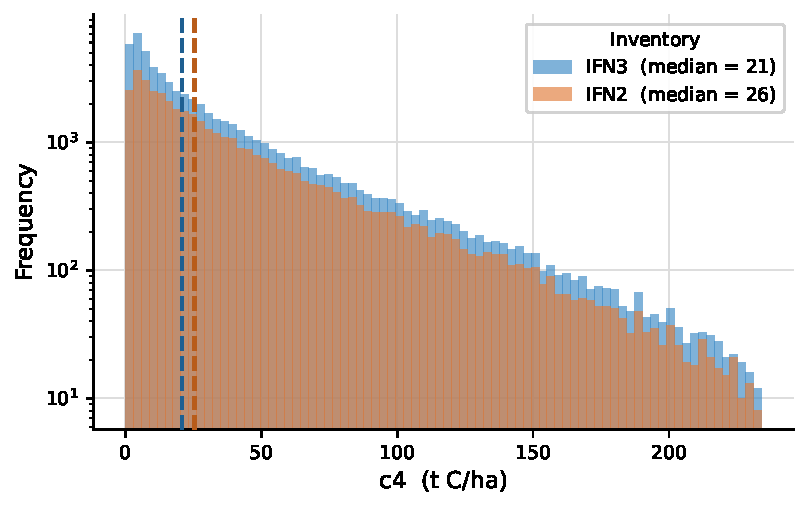
\includegraphics[width=\textwidth]{figuras/06_desarrollo_modelo/hist_c4.pdf}
        \caption{Histogram of the \texttt{c4} variable on a logarithmic scale.}
        \label{fig:hist_c4_sub}
    \end{subfigure}
    \hfill
    \begin{subfigure}{0.48\textwidth}
        \centering
        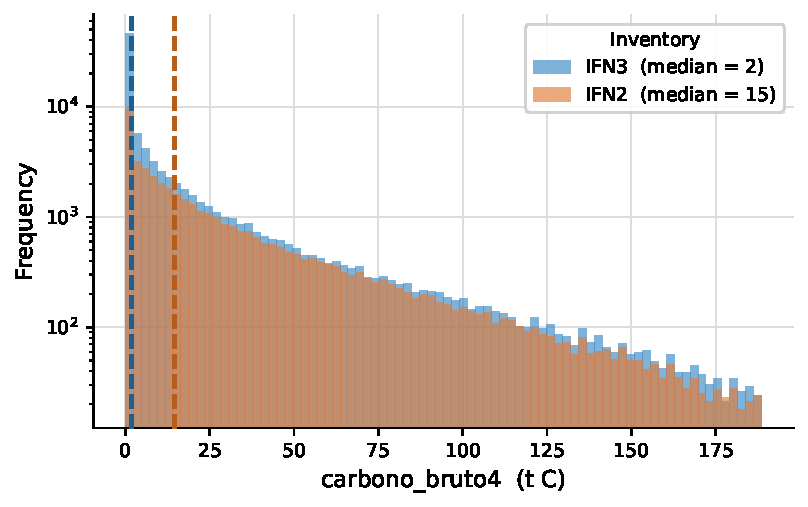
\includegraphics[width=\textwidth]{figuras/06_desarrollo_modelo/hist_carbono_bruto4.pdf}
        \caption{Histogram of the \texttt{carbono\_bruto4} variable on a logarithmic scale.}
        \label{fig:hist_carbono_bruto4_sub}
    \end{subfigure}
    \caption{Histogram of the \texttt{c4} and \texttt{carbono\_bruto4} variables in the cleaned dataset.}
    \label{fig:histograma_datos_combinado}
\end{figure}

On the other hand, Figure \ref{fig:distribucion_variables_combinado} shows the distributions of the target variables separated by inventory. It can be observed that the histogram of the \texttt{carbono\_bruto4} variable is notably more concentrated at low values than that corresponding to \texttt{c4}, for which the amount of carbon has been standardised per unit area.

\begin{figure}
    \centering
    \begin{subfigure}{0.48\textwidth}
        \centering
        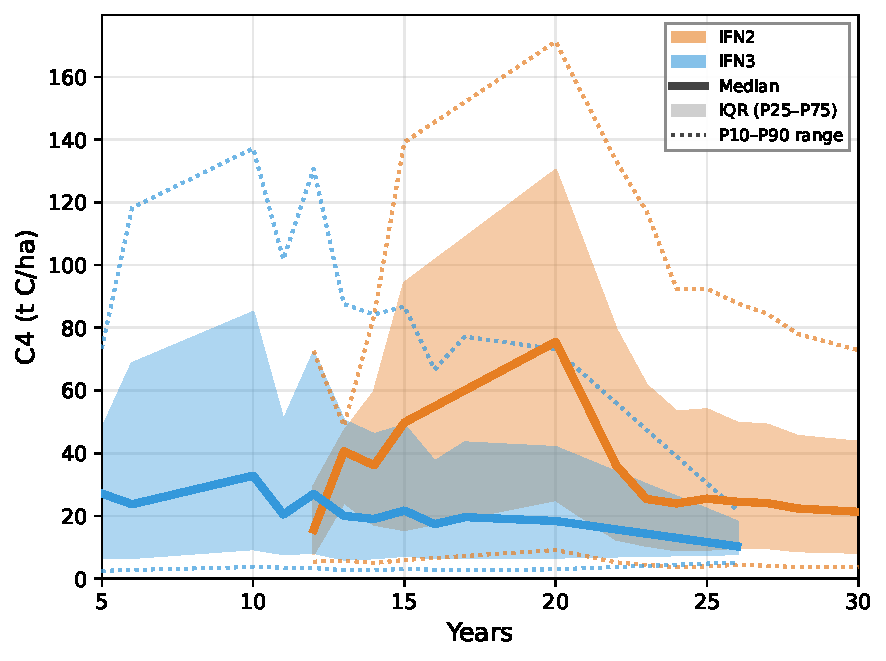
\includegraphics[width=\textwidth]{figuras/06_desarrollo_modelo/ribbon_c4.pdf}
        \caption{Distribution of the \texttt{c4} variable across values of the \texttt{periodo\_agrupado} variable.}
        \label{fig:distribucion_c4_sub}
    \end{subfigure}
    \hfill
    \begin{subfigure}{0.48\textwidth}
        \centering
        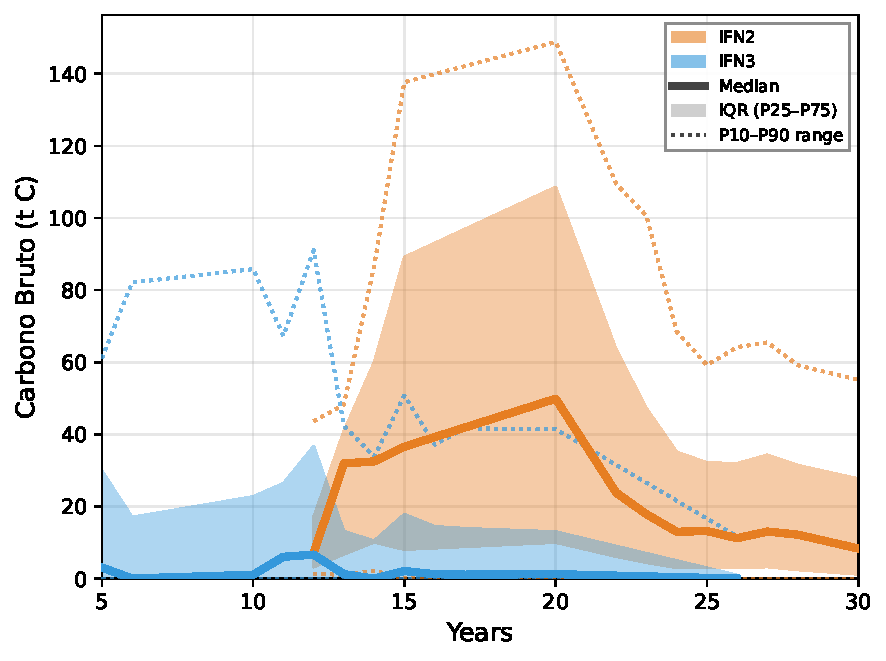
\includegraphics[width=\textwidth]{figuras/06_desarrollo_modelo/ribbon_carbono_bruto4.pdf}
        \caption{Distribution of the \texttt{carbono\_bruto4} variable across values of the \texttt{periodo\_agrupado} variable.}
        \label{fig:distribucion_carbono_bruto4_sub}
    \end{subfigure}
    \caption{Distribution of the \texttt{c4} and \texttt{carbono\_bruto4} variables in the cleaned dataset (after applying filters) separated by inventory.}
    \label{fig:distribucion_variables_combinado}
\end{figure}


\subsubsection{Effect of the period on carbon}
\label{subsec:resultados_periodo_anova}

The influence of \textit{periodo} on the carbon variables was evaluated
using one-way ANOVA. The analyses carried out
show that \textit{periodo} has a significant effect on both
variables. For \texttt{c4}, a test statistic of
\(F = 143.49\) \((p < 0.001)\) was obtained, while for \texttt{carbono\_bruto4}
the value was \(F = 161.08\) \((p < 0.001)\).
These results indicate that the differences observed between periods
are not random, but reflect systematic variations associated with the
sampling time, confirming that \textit{periodo} constitutes a
relevant explanatory factor in the dynamics of forest carbon.

% !TEX root = ../main_final_en.tex
\section{Results}
\label{sec:resultados}

The following presents the results obtained on the test dataset, organised by source inventory (IFN2, IFN3 or IFN2$+$IFN3) and target variable (carbon in tC/ha or total tC). For each combination, the three best base models and the three best stacking ensemble models are shown, ordered by descending $R^2$. The left column indicates the evaluation inventory, i.e., the inventory on which the predictions were made. When a model carries the subscript \textit{global}, it indicates that it was trained with the combined IFN2$+$IFN3 data, even if it was evaluated on a single inventory. Models without a subscript were trained exclusively on the inventory on which they were evaluated.


The complete tables with all evaluated models are included in Appendix~\ref{anexo:resultados}.

\begin{table*}[htbp]
    \centering
    \caption{Top-3 base and \textit{stacking} models by source inventory and target variable, ordered by descending $R^2$. Models with the subscript \textit{global} were trained with combined IFN2$+$IFN3 data.}
    \label{tab:top3_modelos}
    \small
    \renewcommand{\arraystretch}{1.1}
    \begin{tabular}{cclcrrr}
        \toprule
        \textbf{Evaluation inventory} & \textbf{\#} & \textbf{Model} & \textbf{Type} & $\boldsymbol{R^2}$ & \textbf{RMSE} & \textbf{MAE} \\
        \midrule
        \multicolumn{7}{l}{\textit{Target variable: \texttt{c4} (tC/ha)}} \\
        \midrule
        \multirow{6}{*}{IFN2}
            & 1 & LightGBM$_{\text{global}}$             & Base     & 0.719 & 26.806 & 14.689 \\
            & 2 & LightGBM                               & Base     & 0.712 & 26.435 & 14.755 \\
            & 3 & CatBoost$_{\text{global}}$             & Base     & 0.708 & 27.359 & 14.832 \\
        \cmidrule{2-7}
            & 1 & Stack5 GradientBoosting                & Stacking & 0.724 & 25.889 & 14.531 \\
            & 2 & Stack1 MLP$_{\text{global}}$           & Stacking & 0.722 & 26.683 & 14.582 \\
            & 3 & Stack2 MLP$_{\text{global}}$           & Stacking & 0.721 & 26.726 & 14.475 \\
        \cmidrule{1-7}
        \multirow{6}{*}{IFN3}
            & 1 & LightGBM                               & Base     & 0.858 & 17.816 &  9.246 \\
            & 2 & XGBoost                                & Base     & 0.851 & 18.232 &  9.203 \\
            & 3 & CatBoost                               & Base     & 0.849 & 18.385 &  9.746 \\
        \cmidrule{2-7}
            & 1 & Stack4 GradientBoosting                & Stacking & 0.866 & 17.303 &  9.134 \\
            & 2 & Stack5 GradientBoosting                & Stacking & 0.865 & 17.369 &  9.037 \\
            & 3 & Stack2 GradientBoosting                & Stacking & 0.863 & 17.537 &  9.097 \\
        \cmidrule{1-7}
        \multirow{6}{*}{IFN2$+$IFN3}
            & 1 & LightGBM$_{\text{global}}$             & Base     & 0.787 & 22.767 & 11.650 \\
            & 2 & XGBoost$_{\text{global}}$              & Base     & 0.784 & 22.952 & 11.590 \\
            & 3 & CatBoost$_{\text{global}}$             & Base     & 0.783 & 22.990 & 11.607 \\
        \cmidrule{2-7}
            & 1 & Stack5 MLP$_{\text{global}}$           & Stacking & 0.794 & 22.387 & 11.321 \\
            & 2 & Stack2 MLP$_{\text{global}}$           & Stacking & 0.794 & 22.405 & 11.403 \\
            & 3 & Stack4 MLP$_{\text{global}}$           & Stacking & 0.792 & 22.527 & 11.314 \\
        \midrule
        \multicolumn{7}{l}{\textit{Target variable: \texttt{carbono\_bruto4} (tC)}} \\
        \midrule
        \multirow{6}{*}{IFN2}
            & 1 & CatBoost$_{\text{global}}$             & Base     & 0.765 & 18.533 & 10.402 \\
            & 2 & LightGBM$_{\text{global}}$             & Base     & 0.762 & 18.627 & 10.417 \\
            & 3 & XGBoost$_{\text{global}}$              & Base     & 0.762 & 18.644 & 10.428 \\
        \cmidrule{2-7}
            & 1 & Stack5 MLP$_{\text{global}}$           & Stacking & 0.768 & 18.405 & 10.210 \\
            & 2 & Stack5 LinearReg.$_{\text{global}}$      & Stacking & 0.768 & 18.418 & 10.306 \\
            & 3 & Stack4 MLP$_{\text{global}}$           & Stacking & 0.767 & 18.433 & 10.229 \\
        \cmidrule{1-7}
        \multirow{6}{*}{IFN3}
            & 1 & LightGBM                               & Base     & 0.898 & 10.641 &  4.687 \\
            & 2 & CatBoost                               & Base     & 0.896 & 10.737 &  4.789 \\
            & 3 & XGBoost                                & Base     & 0.895 & 10.761 &  4.713 \\
        \cmidrule{2-7}
            & 1 & Stack4 MLP                             & Stacking & 0.902 & 10.407 &  4.517 \\
            & 2 & Stack5 GradientBoosting                & Stacking & 0.901 & 10.433 &  4.540 \\
            & 3 & Stack5 MLP                             & Stacking & 0.901 & 10.447 &  4.454 \\
        \cmidrule{1-7}
        \multirow{6}{*}{IFN2$+$IFN3}
            & 1 & CatBoost$_{\text{global}}$             & Base     & 0.845 & 13.846 &  6.615 \\
            & 2 & LightGBM$_{\text{global}}$             & Base     & 0.841 & 14.006 &  6.654 \\
            & 3 & XGBoost$_{\text{global}}$              & Base     & 0.840 & 14.054 &  6.655 \\
        \cmidrule{2-7}
            & 1 & Stack5 MLP$_{\text{global}}$           & Stacking & 0.847 & 13.756 &  6.399 \\
            & 2 & Stack4 MLP$_{\text{global}}$           & Stacking & 0.847 & 13.766 &  6.429 \\
            & 3 & Stack4 Lin.Reg.$_{\text{global}}$      & Stacking & 0.846 & 13.782 &  6.533 \\
        \bottomrule
    \end{tabular}
\end{table*}

\clearpage
% !TEX root = ../main_final_en.tex
\section{Discussion}
\label{sec:discusion}

First, the ``global'' models will be analysed, i.e., those trained on all data (IFN2 and IFN3) simultaneously. Subsequently, models trained on a single inventory will be analysed and compared with the global ones.


\subsection{Global models}

\subsubsection{Variable \texttt{c4} (in tonnes of carbon per hectare)}
\vspace{0.3cm}
\paragraph{Base models}

The variable \texttt{periodo} (the number of years between the measurement and the prediction) is of great importance in the study of the models. For this reason, Figure \ref{fig:LightGBM_rmse_y_pct_rmse_cuantiles} includes metrics as a function of this variable, showing the evolution of RMSE and \%RMSE in quantiles as a function of the \texttt{periodo} variable, together with a histogram that allows visualisation of the amount of data in the training set for each value of \texttt{periodo}.

\begin{figure*}[htbp]
    \centering
    \begin{subfigure}[b]{0.48\linewidth}
        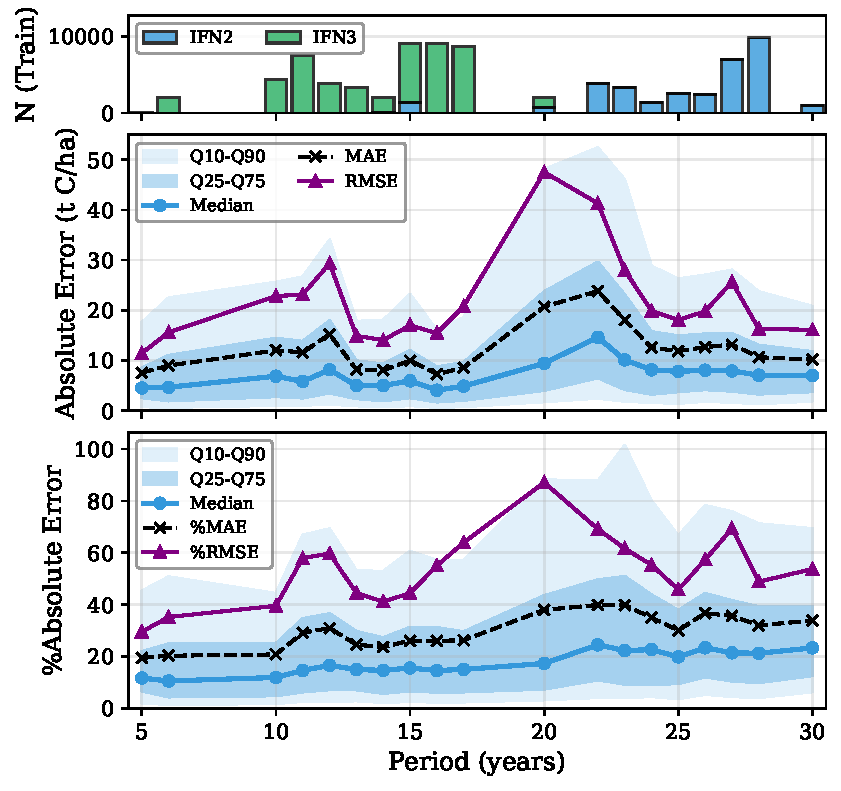
\includegraphics[width=\linewidth]{figuras/09_discusion/c4_LightGBM_metrics.pdf}
        \caption{LightGBM$_{\text{global}}$, \texttt{c4} (tC/ha).}
        \label{fig:LightGBM_rmse_y_pct_rmse_cuantiles}
    \end{subfigure}
    \hfill
    \begin{subfigure}[b]{0.48\linewidth}
        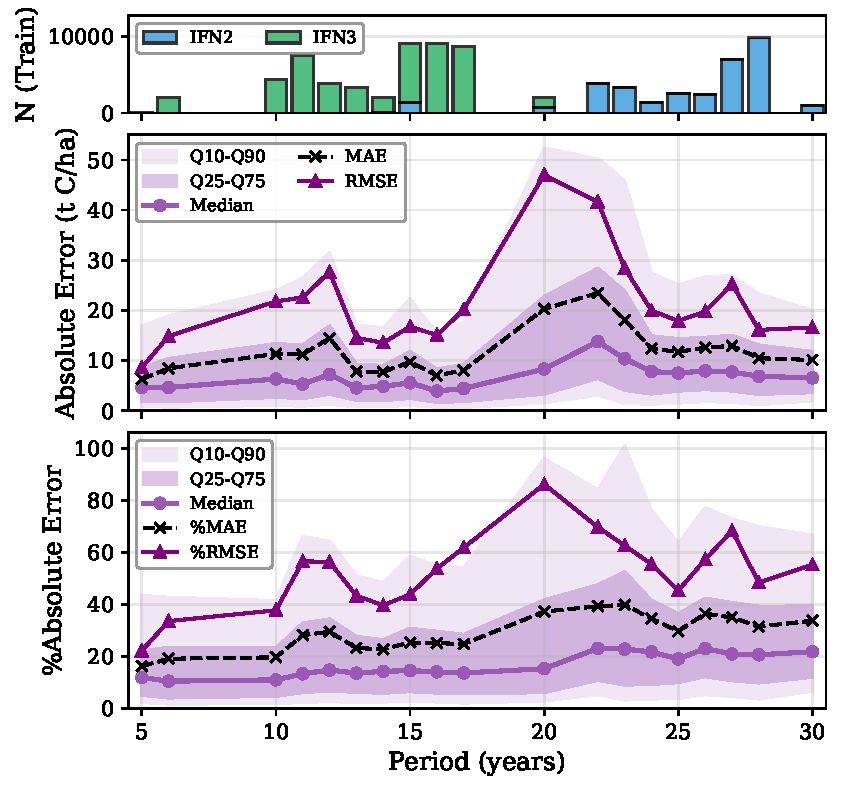
\includegraphics[width=\linewidth]{figuras/09_discusion/c4_Stack5_MLP_metrics.pdf}
        \caption{Global stacking (Conf.~5, MLP), \texttt{c4} (tC/ha).}
        \label{fig:Stack5_MLP_rmse_y_pct_rmse_cuantiles}
    \end{subfigure}
    \\[0.5em]
    \begin{subfigure}[b]{0.48\linewidth}
        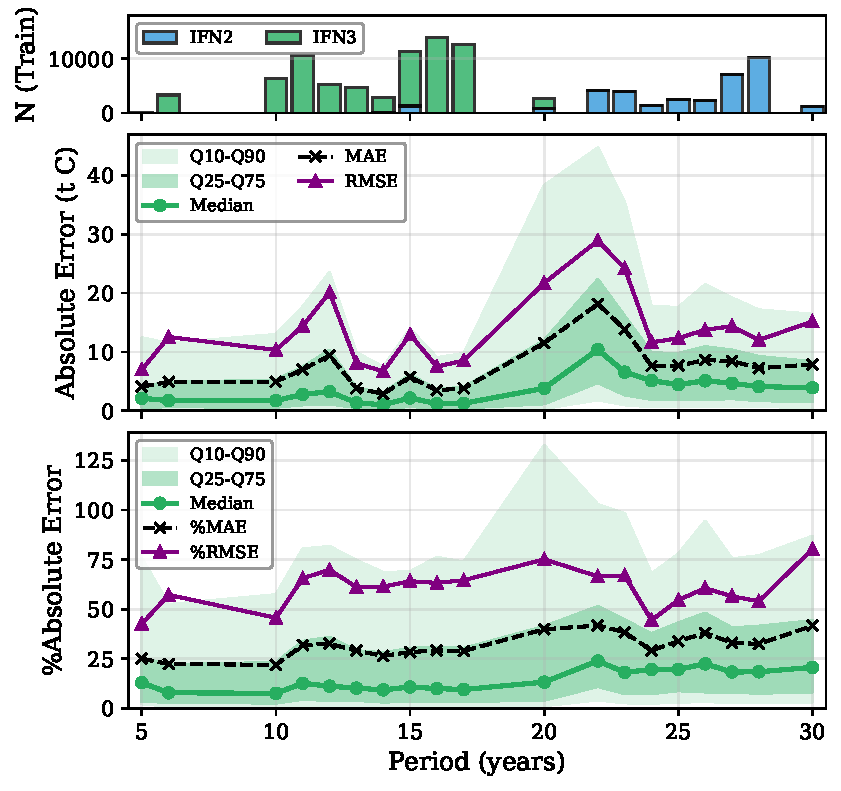
\includegraphics[width=\linewidth]{figuras/09_discusion/carbono_bruto4_CatBoost_metrics.pdf}
        \caption{CatBoost$_{\text{global}}$, \texttt{carbono\_bruto4} (tC).}
        \label{fig:CatBoost_combined}
    \end{subfigure}
    \hfill
    \begin{subfigure}[b]{0.48\linewidth}
        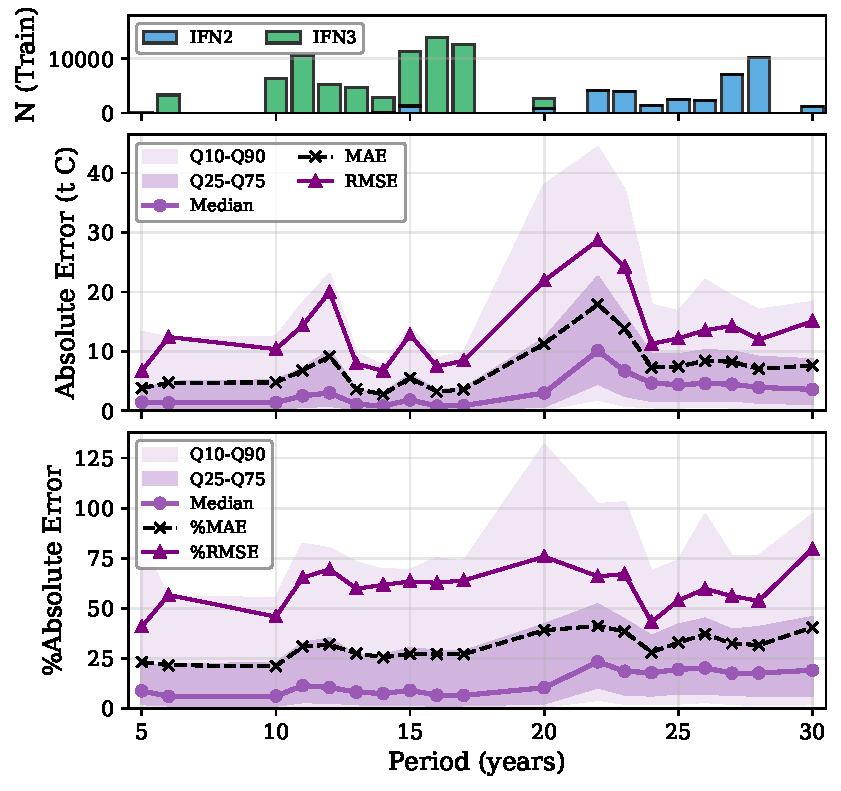
\includegraphics[width=\linewidth]{figuras/09_discusion/carbono_bruto4_Stack5_MLP_metrics.pdf}
        \caption{Global stacking (Conf.~5, MLP), \texttt{carbono\_bruto4} (tC).}
        \label{fig:Stack5_MLP_combined_rmse_y_pct_rmse_cuantiles}
    \end{subfigure}
    \caption{Evolution of absolute error and percentage absolute error in quantiles as a function of the period for the best global models (IFN2$+$IFN3), base and \textit{stacking}, for each target variable.}
    \label{fig:metrics_all}
\end{figure*}

\begin{figure*}[htbp]
    \centering
    \begin{subfigure}[b]{0.48\linewidth}
        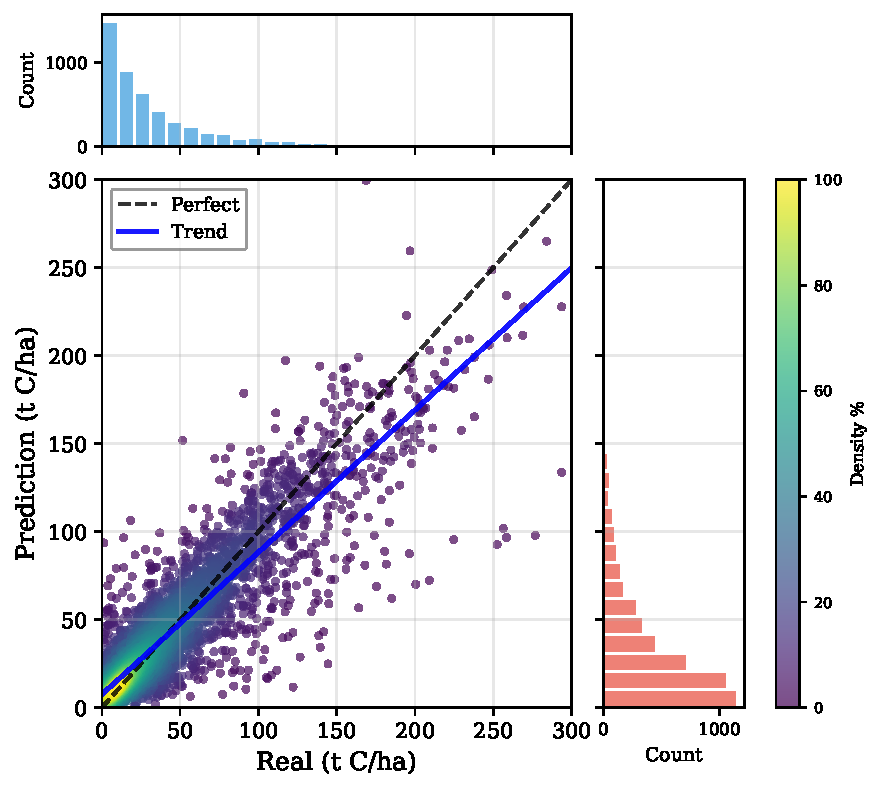
\includegraphics[width=\linewidth]{figuras/09_discusion/c4_LightGBM_density.pdf}
        \caption{LightGBM$_{\text{global}}$, \texttt{c4} (tC/ha).}
        \label{fig:density_LightGBM_0-300}
    \end{subfigure}
    \hfill
    \begin{subfigure}[b]{0.48\linewidth}
        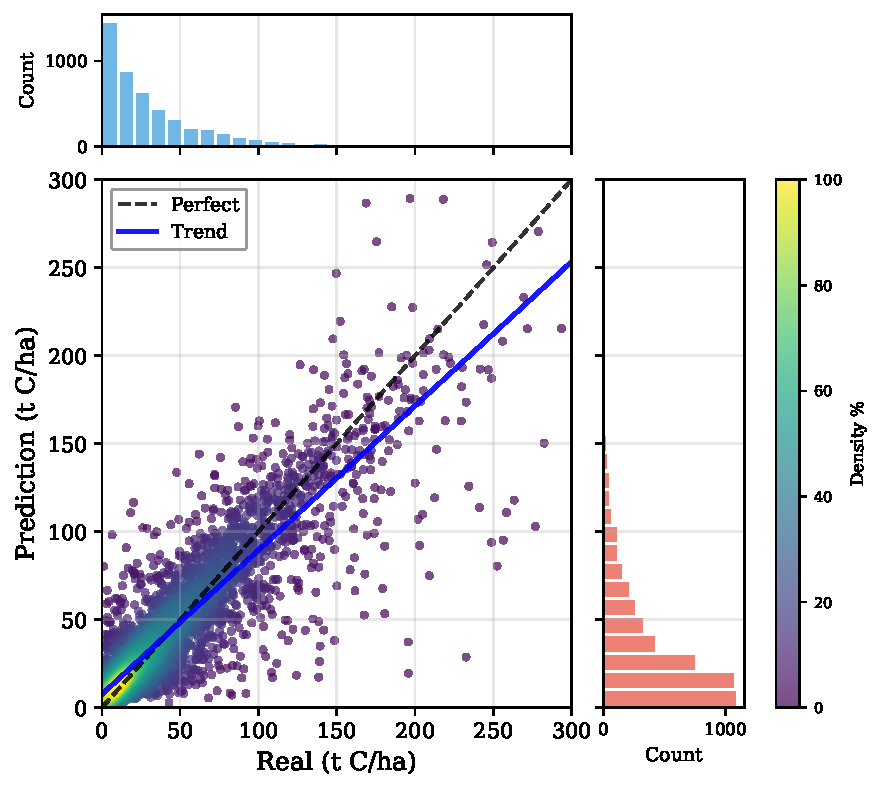
\includegraphics[width=\linewidth]{figuras/09_discusion/c4_Stack5_MLP_density.pdf}
        \caption{Global stacking (Conf.~5, MLP), \texttt{c4} (tC/ha).}
        \label{fig:Stack5_MLP_density}
    \end{subfigure}
    \\[0.5em]
    \begin{subfigure}[b]{0.48\linewidth}
        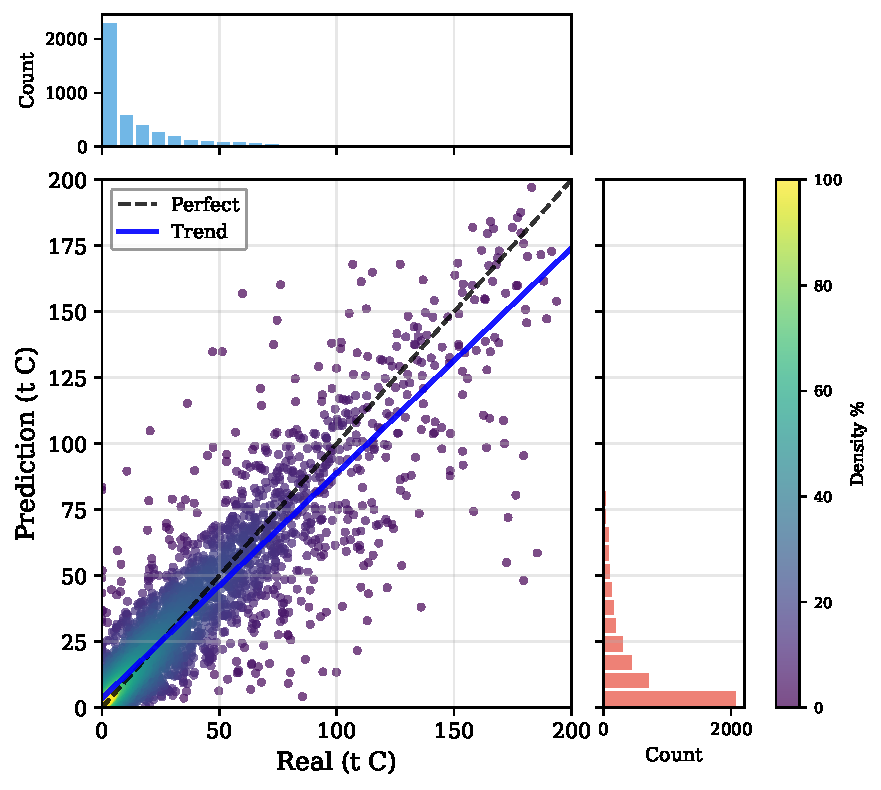
\includegraphics[width=\linewidth]{figuras/09_discusion/carbono_bruto4_CatBoost_density.pdf}
        \caption{CatBoost$_{\text{global}}$, \texttt{carbono\_bruto4} (tC).}
        \label{fig:CatBoost_density}
    \end{subfigure}
    \hfill
    \begin{subfigure}[b]{0.48\linewidth}
        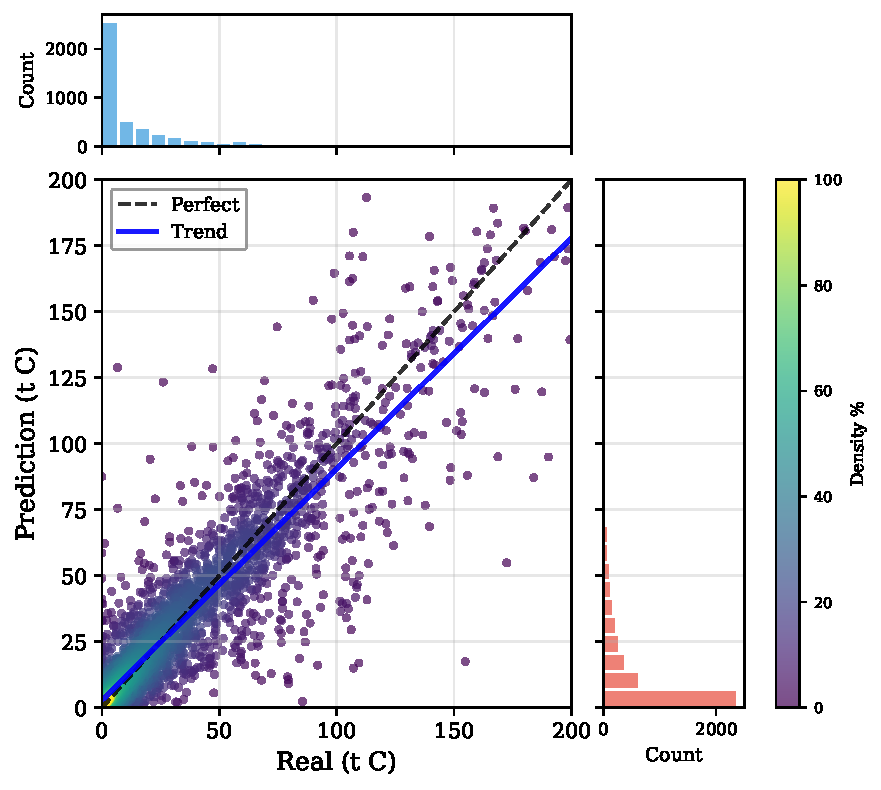
\includegraphics[width=\linewidth]{figuras/09_discusion/carbono_bruto4_Stack5_MLP_density.pdf}
        \caption{Global stacking (Conf.~5, MLP), \texttt{carbono\_bruto4} (tC).}
        \label{fig:Stack5_MLP_density_carbono_bruto4}
    \end{subfigure}
    \caption{Prediction density versus actual values for the best global models (IFN2$+$IFN3), base and \textit{stacking}, for each target variable.}
    \label{fig:density_all}
\end{figure*}

% Tanto en la Figura \ref{fig:LightGBM_rmse_cuantiles} como en la Figura \ref{fig:LightGBM_rmse_porcentual_cuantiles} se observa el mismo comportamiento: las mejores predicciones se obtienen en aquellos casos en los que los datos de entrenamiento provienen del IFN3. Esto se ve claramente en la forma en la que aumentan los errores (sobre todo los del cuantil $90$) cuando se intenta predecir valores para un periodo mayor a $17$ años, valor a partir del cuál los datos del IFN3 se acaban. Observamos que a partir de los $17$ años aumentan en gran medida los valores grandes de error (cuantil $90$) junto con los valores grandes - medios (cuantil $75$). No obstante, los valores medianos y los pequeños - medios (cuantil $25$) se mantienen relativamente estables, aumentando ligeramente con el periodo.

We can observe something we could anticipate: the difficulty of prediction depends on a combination of how far into the future the prediction is desired and the quality and quantity of training data. Starting in the IFN3 range, we can observe that for the first years ($5$, and $6$), despite having few data points, errors are modest. As the period increases (between $10$ and $17$ years), mean and median errors remain relatively stable despite generally having more training data. Large extreme errors (quantile $90$) experience a widespread increase. When we enter the range of years where training data come mainly from the IFN2 (the range between $20$ and $30$ years), although the median and the low-to-medium values (quantile $25$) remain stable, the medium-to-high (quantile $75$) and large (quantile $90$) values increase substantially. This indicates that, even with a large amount of training data (especially for years $27$ and $28$), the combination of lower data quality (always comparing with IFN3) and prediction at distant values makes model prediction harder. Furthermore, as can be seen in Figure \ref{fig:distribucion_variables_combinado}, the values for the first years of IFN2 show high variability, being mostly higher than those of IFN3 for the same years, with greater variability. This, combined with the fact that the amount of data for those years is not excessively large, causes the model to obtain worse predictions.

The fact that median values remain relatively stable across all periods indicates that the model correctly assimilates the behaviour of the target variable both with IFN2 and IFN3 data. On the other hand, the high quantile $90$ errors can be explained by several factors: the high variability of the dataset, the smaller number of field variables collected in the IFN2 (which reduces available information) and the greater inherent difficulty of predicting over long time horizons. This combination makes particular or atypical cases less recognisable by the model, especially when they come from the IFN2, where discriminative capacity is lower than in the IFN3. The aforementioned variability is clearly visible in Figure~\ref{fig:density_LightGBM_0-300}, which shows predicted values versus actual values for the model with the best metrics, along with a distribution histogram.

\paragraph{Stacking models}

The incorporation of \textit{stacking} schemes does not produce substantial, though systematic, increases in the coefficient of determination with respect to the best individual models. Looking at Table \ref{tab:stack_global_c4} we can observe that stacking models present better metrics in the vast majority of cases, always compared with the base models. The best parameters are obtained by the stacking model with configuration 5, which retains all models with competitive performance, together with the neural network meta-model.

The fact that all ensembles improve upon the base models is a sign that this improvement is not a statistical exception, but a real improvement. That is, it is not the case that the metrics are better due to stochasticity in the meta-model parameters, but because the stacking genuinely improves the final result. Obviously, retraining the meta-models with other parameters would change the metrics, but the fact is that the function of improving predictions is indeed achieved with the ensembles. However, the improvement is small, which may mean that depending on the case, simplicity of using one of the base models is preferred over one of the ensembles.

Figure \ref{fig:Stack5_MLP_rmse_y_pct_rmse_cuantiles} shows the evolution of RMSE and percentage RMSE in quantiles for the ensemble model with the best metrics, the stacking with configuration 5 and MLP meta-model. We can observe that the behaviour is practically identical to that of LightGBM, which achieved the best metrics among the base models.
On the other hand, in Figure \ref{fig:Stack5_MLP_density} we can see the scatter plot of predictions versus actual values for the stacking model with configuration 5 and MLP meta-model for the variable \texttt{c4} (tC/ha).


Regarding the structure of the ensembles, the best results are obtained when high-quality, similar-nature base models are combined (mainly \textit{gradient boosting} variants) and meta-models of moderate complexity, such as MLP or linear SVR, are used. In contrast, stacks with few base models or those incorporating excessively flexible meta-models, such as Random Forest at the second level, tend to offer lower performance, probably due to the low dimensionality of the meta-predictor space or unnecessary overfitting of residual noise.



\subsubsection{Variable \texttt{carbono\_bruto4} (in tonnes of carbon)}
\vspace{0.3cm}
\paragraph{Base models}

In the same way as in the previous sections, Figure \ref{fig:CatBoost_combined} shows the evolution of RMSE and \%RMSE in quantiles as a function of the \texttt{periodo} variable for the CatBoost model (the one that achieved the best metrics among the base models) with IFN2 and IFN3 as explanatory variables for the variable in tonnes of carbon, together with the histogram of the distribution of training data as a function of the period variable.


Referring to Figure \ref{fig:CatBoost_combined} we observe the same qualitative behaviour as in the case of the \texttt{c4} variable (with the particularity that units and value range change): the error between quantiles $25$ and $75$ remains at relatively small and constant values, although it is true that it starts smaller and gradually increases as the period variable increases. Extreme errors (quantile $90$) remain high. In fact, looking at the highest values of the percentage RMSE for quantile $90$, we observe that notably higher values are reached than in the case of the \texttt{c4} variable, reaching up to $130\%$ when for \texttt{c4} it barely exceeded $100\%$ for the worst case. This is noteworthy, since the global metrics for predictions of the variable \texttt{carbono\_bruto4} (see Table \ref{tab:base_global_carbono_bruto4}) are systematically better than those of the variable \texttt{c4} (see Table \ref{tab:base_global_c4}). That is, the variable \texttt{carbono\_bruto4} (tonnes) is generally easier for models to predict than the variable \texttt{c4} (tonnes per hectare), but the opposite occurs in particular cases, where the highest errors shoot up in a more exaggerated manner than in the same case for the \texttt{c4} variable. The increase in error when moving from the IFN2 to IFN3 year range is also observed, caused by the increase in variability of the second inventory data (see Figure \ref{fig:distribucion_variables_combinado}).

As in the previous sections, Figure \ref{fig:CatBoost_density} shows a scatter plot of predictions versus actual values for the CatBoost model for the case under consideration.




\paragraph{Stacking models}

The results obtained in this section are very similar to those obtained with the stacking models for the \texttt{c4} (tC/ha) variable. That is, we find a systematic improvement in all stacking models over the base models, but that improvement is small. This causes the results to be strictly better, as can be seen in Table \ref{tab:stack_global_carbono_bruto4} compared with the base model metrics in Table \ref{tab:base_global_carbono_bruto4}. Again, the fact that the improvement of stacking models over base models is systematic indicates that we are not facing a statistical incident, but rather that the stacking format is capable of improving predictions by choosing the best decisions from each model. However, as noted above, the complexity of training five models in addition to the meta-model may be inconvenient compared to the possibility of using, for example, the best of the individual models.

The ensemble model that provides the best metrics for predicting the \texttt{carbono\_bruto4} (tC) variable is configuration 5 with an MLP meta-model, as was also the case for the \texttt{c4} (tC/ha) variable. The evolution of RMSE and percentage RMSE in quantiles as a function of the \texttt{periodo} variable for this model can be visualised in Figure \ref{fig:Stack5_MLP_combined_rmse_y_pct_rmse_cuantiles}.



On the other hand, Figure \ref{fig:Stack5_MLP_density_carbono_bruto4} shows a scatter plot of predictions versus actual values for the stacking model with configuration 5, MLP meta-model and the variable \texttt{carbono\_bruto4} (tC).

\subsection{Individual models trained on IFN2 or IFN3 only.}

When comparing the performance of ``global'' models (trained on the combined IFN2 and IFN3 dataset) versus ``local'' models (trained exclusively on IFN2 or IFN3), differentiated behaviour is observed depending on the test inventory. For IFN3, local models outperform global ones in terms of accuracy metrics. Conversely, for IFN2, global models show superior performance.

A possible explanation for this phenomenon lies in the quality and quantity of information contained in each inventory. The IFN2 data, being less informative or having fewer variables, appear to benefit from joint learning with IFN3 data, allowing models to capture additional patterns and improve their generalisation capacity on the second inventory. In contrast, for IFN3, whose data possess higher intrinsic quality, the inclusion of IFN2 records during training could be introducing noise or unwanted variability, which ultimately penalises the accuracy of the final model predictions on this dataset.

\begin{figure*}[htbp]
    \centering
    \begin{subfigure}[b]{0.48\linewidth}
        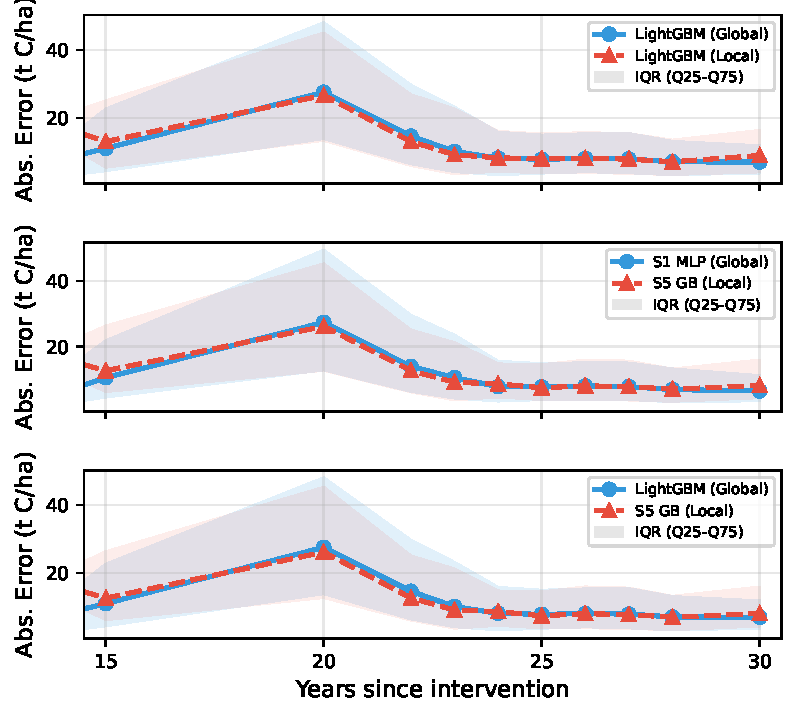
\includegraphics[width=\linewidth]{figuras/09_discusion/Consolidado_IFN2_c4_clean.pdf}
        \caption{IFN2, \texttt{c4} (tC/ha).}
        \label{fig:comparativa_mejores}
    \end{subfigure}
    \hfill
    \begin{subfigure}[b]{0.48\linewidth}
        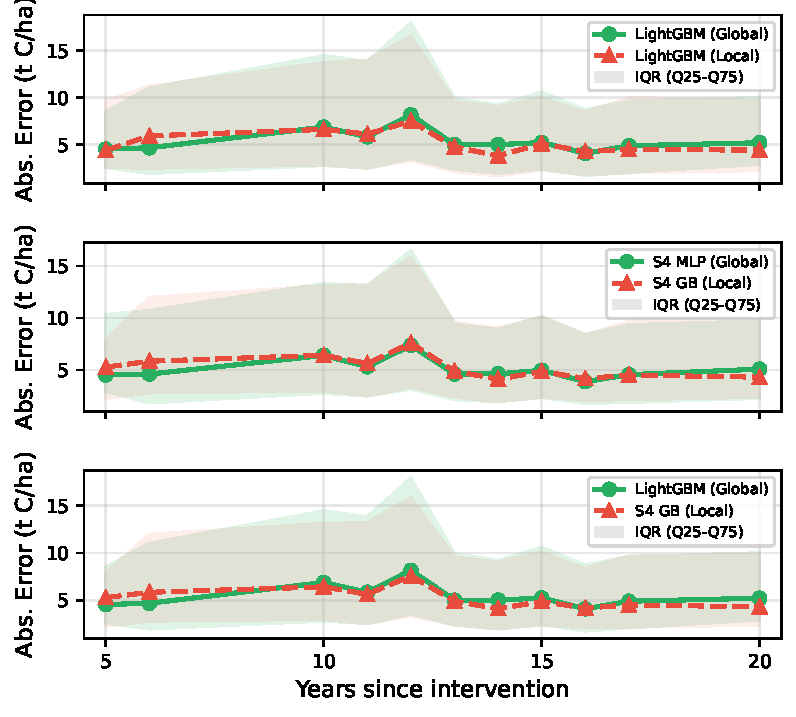
\includegraphics[width=\linewidth]{figuras/09_discusion/Consolidado_IFN3_c4_clean.pdf}
        \caption{IFN3, \texttt{c4} (tC/ha).}
        \label{fig:disc_sub2}
    \end{subfigure}
    \\[0.5em]
    \begin{subfigure}[b]{0.48\linewidth}
        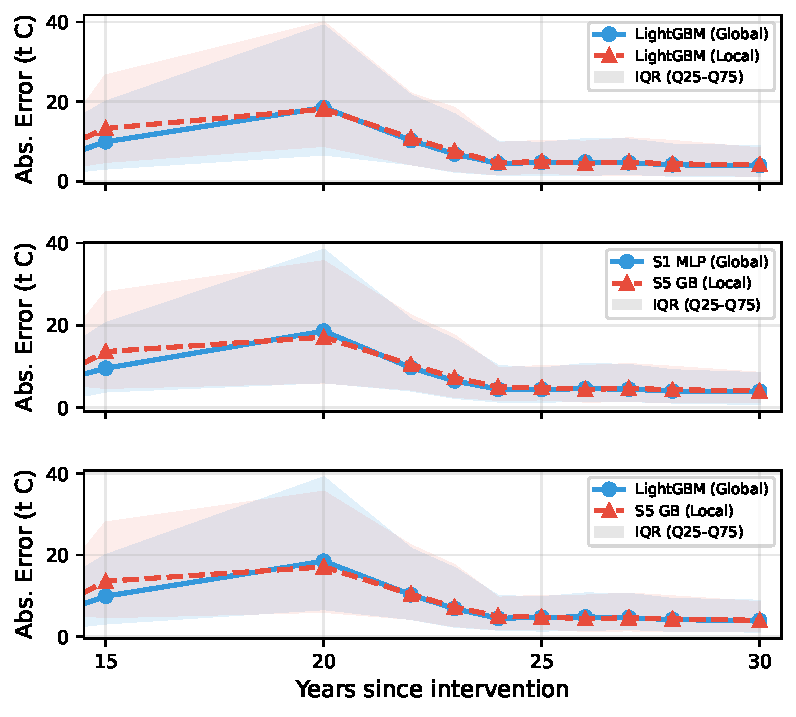
\includegraphics[width=\linewidth]{figuras/09_discusion/Consolidado_IFN2_carbono_bruto4_clean.pdf}
        \caption{IFN2, \texttt{carbono\_bruto4} (tC).}
        \label{fig:disc_sub3}
    \end{subfigure}
    \hfill
    \begin{subfigure}[b]{0.48\linewidth}
        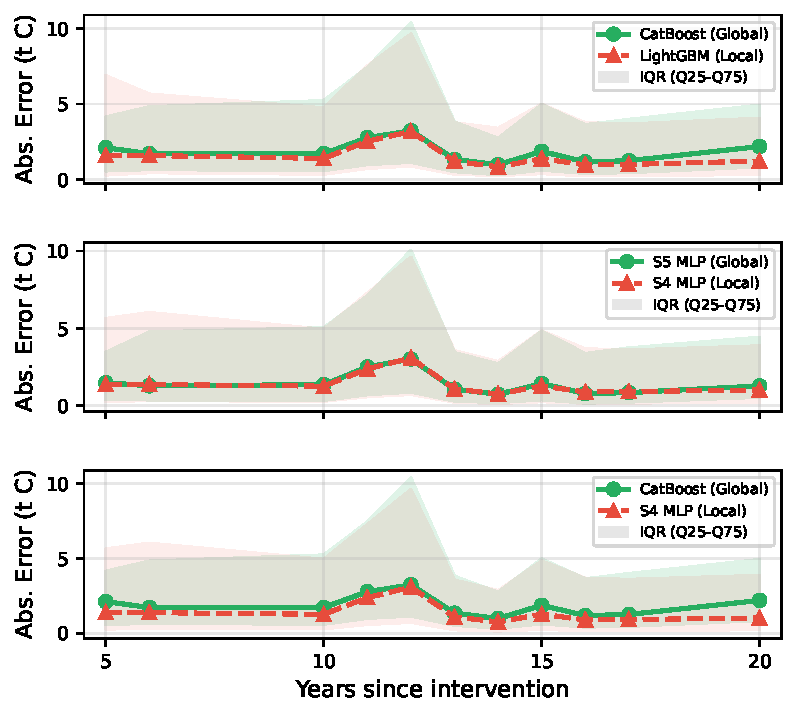
\includegraphics[width=\linewidth]{figuras/09_discusion/Consolidado_IFN3_carbono_bruto4_clean.pdf}
        \caption{IFN3, \texttt{carbono\_bruto4} (tC).}
        \label{fig:disc_sub4}
    \end{subfigure}
    \caption{Comparison of absolute error by inventory and target variable: best global vs.\ local base models, global vs.\ local stacking models, and best base model vs.\ best stacking model.}
    \label{fig:consolidado_all}
\end{figure*}

Figure \ref{fig:comparativa_mejores} shows a comparison between the best global vs.\ local base models (top), best global vs.\ local stacking models (middle) and best base model vs.\ best stacking model (bottom). We observe that in general the lower errors for IFN2 are committed by the global models, while for IFN3 it is the local models that do the better job.


% \subsubsection{Comportamiento global de los modelos}

\subsubsection{Assimilation of target variable behaviour}

With the metrics we have set out and the analysis carried out in this section, it seems clear that, while the results are far from perfect, the models are capable of understanding the logic and meaning of each variable to obtain a prediction with a degree of accuracy that depends on the nature of the instance in question. Another test we can perform to check whether the model results are logical is the one shown in Figures \ref{fig:sensibilidad_escenarios} and \ref{fig:sensibilidad_escenarios_carbono_bruto4}.
These figures show the evolution of several particular cases as time progresses between measurement and prediction. The selected cases are real within the available data. They were selected with the aim of showing how the models behave for more or less common initial carbon configurations. To this end, for each data instance, the \texttt{npies_x} variables were summed, and then the values closest to percentiles 10, 35, 65 and 90 for the resulting variable were selected. This avoids potential problems arising from selecting unrealistic examples.


\begin{figure}
      \centering
      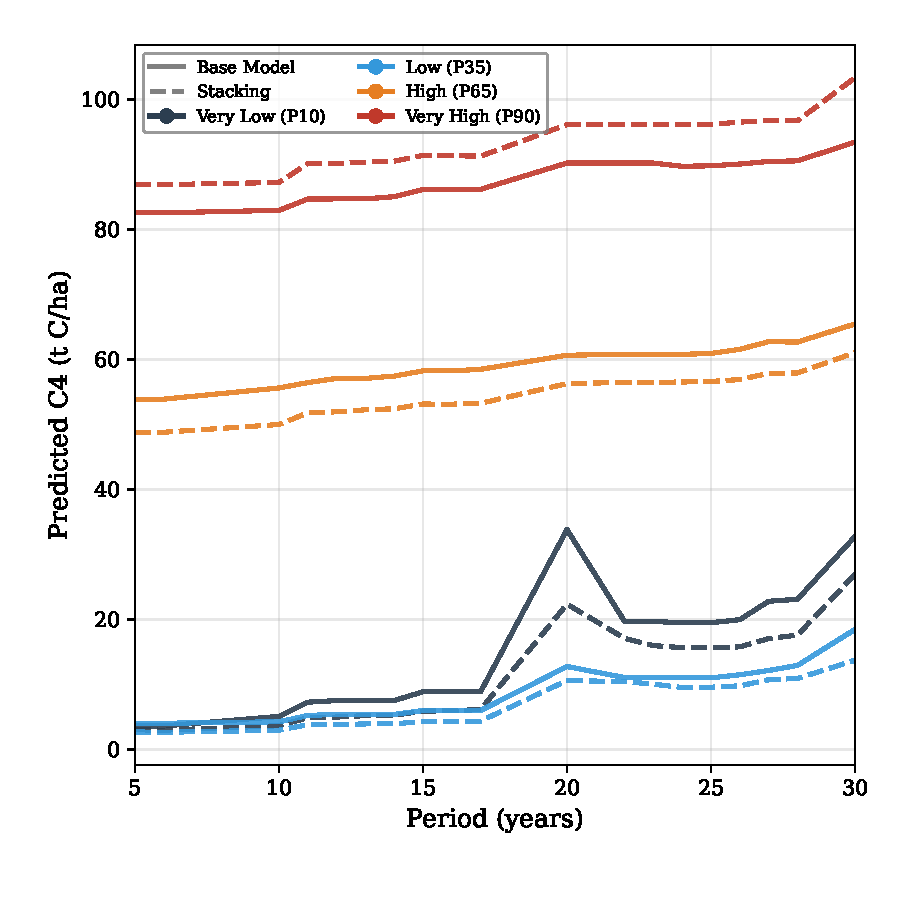
\includegraphics[width=\linewidth]{figuras/09_discusion/sensibilidad_escenarios_c4_P10_P35_P65_P90.pdf}
      \caption{Evolution of the amount of carbon in tonnes per hectare (\texttt{c4}) for several scenarios.}
      \label{fig:sensibilidad_escenarios}
\end{figure}

\begin{figure}
      \centering
      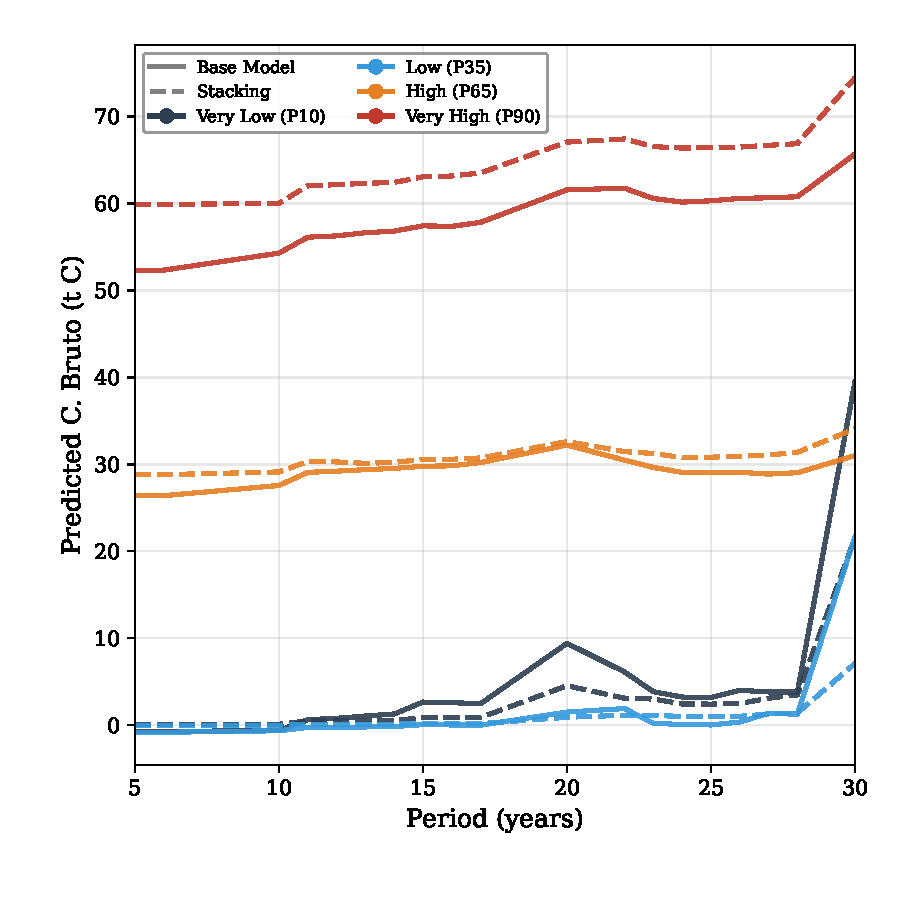
\includegraphics[width=\linewidth]{figuras/09_discusion/sensibilidad_escenarios_carbono_bruto4_P10_P35_P65_P90.pdf}
      \caption{Evolution of the amount of carbon in tonnes (\texttt{carbono\_bruto4}) for several scenarios.}
      \label{fig:sensibilidad_escenarios_carbono_bruto4}
\end{figure}

We can highlight the following features:
\begin{itemize}
      \item The lines of the base models and ensembles for each case are very close together, which is consistent with the obtained metrics, which were very similar to each other.
      \item The general trend is upward, i.e., the models correctly capture the behaviour of tree growth over time for the studied years.
      \item In year $17$ there is a widespread abrupt increase, which is more exaggerated the smaller the percentile of the case study. This is easy to understand by looking at the data, since the values of the variable to be predicted experience a generalised increase when moving from the IFN2 years to those of the IFN3, as can be seen in Figure \ref{fig:distribucion_variables_combinado}. This change (where the model begins to ingest IFN2 data instead of IFN3 data) occurs mainly in year $17$. This can be seen in the histogram of Figure \ref{fig:Stack5_MLP_combined_rmse_y_pct_rmse_cuantiles}, for example. The reason why the jump occurs at small percentiles is that these small values in the IFN2 data barely exist or are less common. The model has seen that for those years carbon values are, in general, higher, and that is what it predicts. In fact, Figure \ref{fig:distribucion_variables_combinado} shows that for the initial years of the IFN2 data, carbon values increase and then decrease, and this is exactly what we see in the predictions: an increase followed by a decrease.
      \item We can also see an abrupt increase in many cases when moving from year $29$ to $30$, especially in the case of the variable in tonnes of raw carbon (Figure \ref{fig:sensibilidad_escenarios_carbono_bruto4}). These years coincide with a scarcity of data, as can be seen in the histogram of Figure \ref{fig:distribucion_variables_combinado}. It is to be expected that predictions for those years will be less reliable, especially for an extreme value.
\end{itemize}


\subsubsection{Model performance as a function of the target variable value}

If we analyse the global metrics in the tables of Section \ref{sec:resultados}, we notice that RMSE values are notably larger than MAE values, specifically around twice as large in most cases. Because RMSE penalises large errors much more heavily than MAE, this is indicative of the presence of outliers in the error. We have already seen throughout this section that the largest errors occur in the range of years in which the IFN2 is the main data source, as can be seen in Figures \ref{fig:LightGBM_rmse_y_pct_rmse_cuantiles}, \ref{fig:Stack5_MLP_rmse_y_pct_rmse_cuantiles}, \ref{fig:CatBoost_combined} and \ref{fig:Stack5_MLP_combined_rmse_y_pct_rmse_cuantiles}, and the main conclusion is that the quality or quantity of information contained in this inventory is inferior. However, this does not fully answer the question of in which cases the model predicts best, beyond the obvious fact that prediction will be better the closer in time and the more data available for that year. This is why Figures \ref{fig:SMAPE_RMSE_deciles_c4_carbono_bruto4} and \ref{fig:distribucion_carbono_bruto4_combinado} can be useful. These figures show the distribution of errors, specifically RMSE and SMAPE, as a function of the target variable for \texttt{c4} and \texttt{carbono\_bruto4} respectively, in deciles for the base models.

\begin{figure}
      \centering
      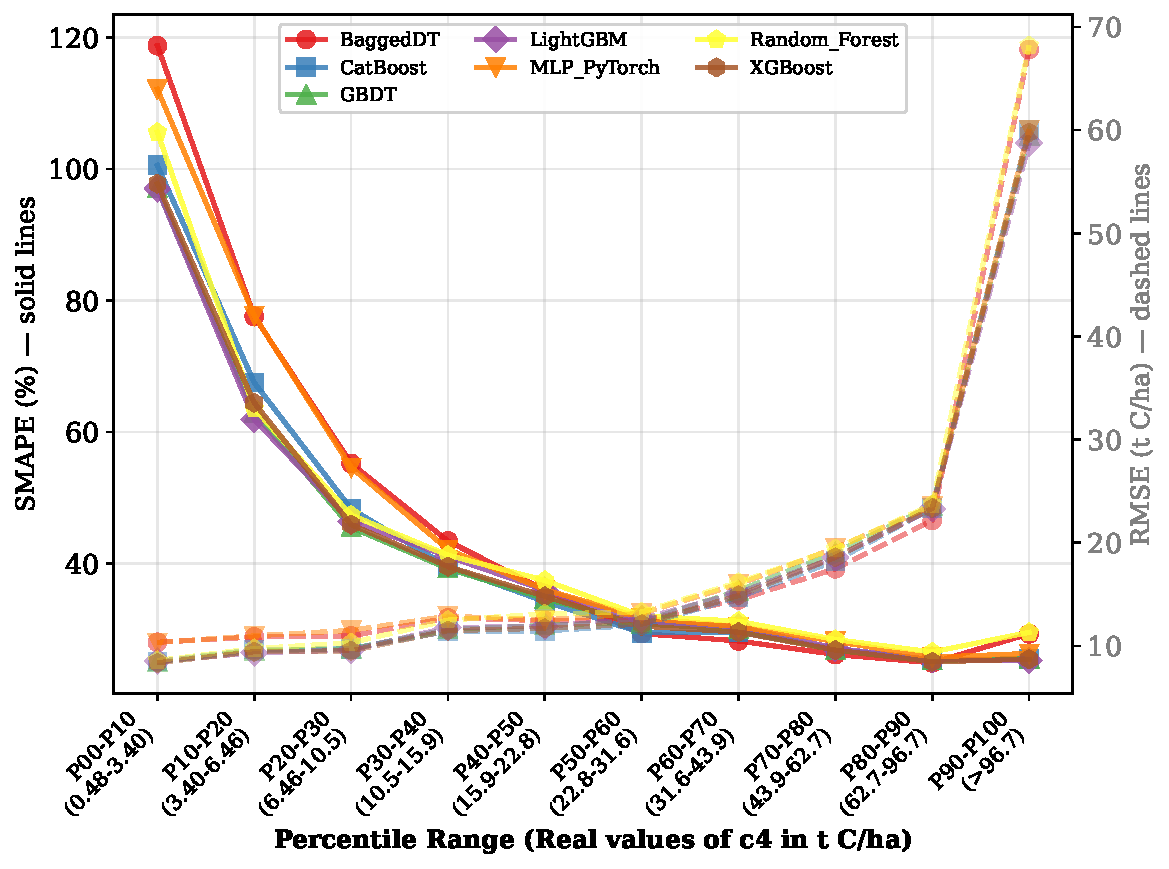
\includegraphics[width=\linewidth]{figuras/09_discusion/c4_base_models_SMAPE_RMSE_percentiles.pdf}
      \caption{Distribution of SMAPE and RMSE as a function of the target variable for \texttt{c4} in deciles.}
      \label{fig:SMAPE_RMSE_deciles_c4_carbono_bruto4}
\end{figure}

\begin{figure}
      \centering
      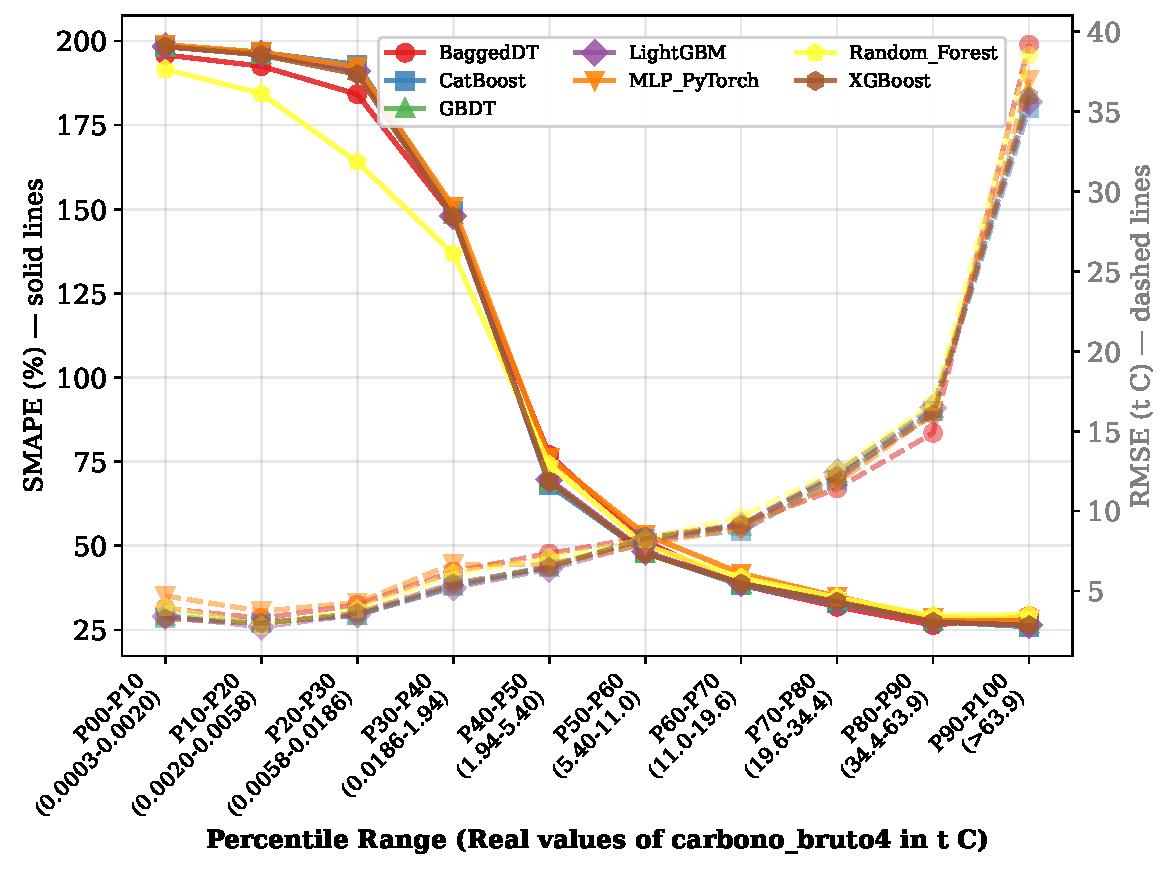
\includegraphics[width=\linewidth]{figuras/09_discusion/carbono_bruto4_base_models_SMAPE_RMSE_percentiles.pdf}
      \caption{Distribution of SMAPE and RMSE as a function of the target variable for \texttt{carbono\_bruto4} in deciles.}
      \label{fig:distribucion_carbono_bruto4_combinado}
\end{figure}


We quickly notice the following: predictions for small values of the target carbon (first deciles) are poor (large SMAPE) despite having the smallest absolute error (small RMSE). Then, as the target carbon increases, RMSE increases slightly while SMAPE decreases much more rapidly, reaching values close to $25\%$. In both cases the best results are achieved when the target carbon is larger, despite a significant increase in RMSE between the second-to-last and last decile. Since this occurs for all models, it suggests that prediction difficulty is not homogeneous across all situations or amounts of carbon, and that despite the lowest-carbon percentiles having the smallest RMSE, model accuracy is not sufficient to make a decent prediction in situations with little biomass. This was predictable, since a larger absolute error for a larger forest plot does not necessarily imply a worse relative error.

Also noteworthy is the fact that the initial deciles have very close carbon ranges, especially for the \texttt{carbono\_bruto4} variable, where the first decile ranges from $0.0003$~tC to $0.0020$~tC. This large number of values with such small carbon does not help models obtain a good prediction. The higher densities at small carbon values are clearly visible in Figures \ref{fig:density_LightGBM_0-300}, \ref{fig:Stack5_MLP_density}, \ref{fig:CatBoost_density} and \ref{fig:Stack5_MLP_density_carbono_bruto4}.

\subsection{Model interpretability: SHAP analysis}
\label{sec:interpretabilidad_shap}

Thanks to the SHAP value analysis we can add explainability to the models, finding out which variables the model gives more importance to and in which cases these values cause the carbon prediction to be higher or lower. In Table \ref{tab:shap_rank_abs} we can observe the mean importance rank of variables with the highest absolute SHAP value, both averaged across all cases (first column ``Mean'') and by source inventory and target variable. In this table we see that the most consistently important variables are \texttt{npies}, \texttt{especie\_id}, \texttt{ocupa} and \texttt{radio}, i.e., variables purely related to the forest structure. The rest of the variables in the table have more variability across the different configurations, where meteorological variables (which appear to be more important than the climatic variable we added, the Martonne index) and edaphic variables are mainly interleaved.

% ============================================================
% Tabla: Ranking medio de variables por |SHAP|
% ============================================================
\begin{table*}[htbp]
  \centering
  \footnotesize
  \caption{Mean SHAP rank per variable across LightGBM, XGBoost, CatBoost, GBDT and MLP (n=2000 samples; rank 1 = most important).}
  \label{tab:shap_rank_abs}
  \begin{tabular}{lccccccc}
    \toprule
    Variable & \textbf{Mean} & \makecell{\textbf{IFN2} \\ \textbf{c4}} & \makecell{\textbf{IFN2} \\ \textbf{carbono\_b4}} & \makecell{\textbf{IFN3} \\ \textbf{c4}} & \makecell{\textbf{IFN3} \\ \textbf{carbono\_b4}} & \makecell{\textbf{IFN2+3} \\ \textbf{c4}} & \makecell{\textbf{IFN2+3} \\ \textbf{carbono\_b4}} \\
    \midrule
    npies* (Density) & \textbf{1} & \textbf{1} & \textbf{1} & \textbf{1} & \textbf{1} & \textbf{1} & \textbf{1} \\
    especie\_id* & 2.2 & 2 & 2 & 2.2 & 2.8 & 2.2 & 2.2 \\
    ocupa & 2.9 & 3.2 & 3 & 3 & 2.2 & 2.8 & 3 \\
    radio & 4.2 & 4.2 & 4.2 & 4.2 & 4.2 & 4.2 & 4.4 \\
    gndvi\_mean\_verano & 6.5 & 5.6 & 5 & 7 & 7 & 8 & 6.6 \\
    tipo\_especie* & 7.1 & 11.6 & 8.8 & 4.6 & 5.8 & 6 & 6 \\
    periodo\_agrupado & 8.4 & 13 & 8 & 10.6 & 8.6 & 5.2 & 5 \\
    skt\_mean\_verano & 9.6 & 6.8 & --- & 10.4 & --- & 11.6 & --- \\
    rocosidad\_id* & 11 & 9 & 7.6 & 17.2 & 12 & 10.2 & 9.8 \\
    fccarb & 11.4 & --- & --- & 9 & 10 & 14 & 12.6 \\
    evi\_mean\_primavera & 11.8 & 12 & 10.6 & 13.6 & 11.2 & 13.2 & 10.4 \\
    elevacion & 12.6 & 12.6 & 7.4 & 15.8 & 12.8 & 14.4 & 12.4 \\
    tratmasa\_id* & 13.2 & --- & --- & 8 & 7.2 & 18.8 & 18.8 \\
    estado\_id* & 13.5 & 21.8 & 12.8 & 17.2 & 12.6 & 8.8 & 8 \\
    ndii\_mean\_primavera & 14.5 & 17 & 11.6 & 14.2 & 15.6 & 15.4 & 13.4 \\
    skt\_mean\_primavera & 15.1 & 17.4 & --- & 13.4 & --- & 14.6 & --- \\
    pr\_sum\_otoño & 15.7 & 16.4 & --- & 14.4 & --- & 16.4 & --- \\
    pr\_sum\_primavera & 15.7 & 10.6 & --- & 17.6 & --- & 19 & --- \\
    pr\_sum\_invierno & 16 & 8.6 & --- & 21.8 & --- & 17.6 & --- \\
    martonneidx\_id* & 16.4 & 18.2 & 10.2 & 24.2 & 13.4 & 20.6 & 11.8 \\
    skt\_std\_verano & 18.4 & 13.2 & --- & 22.8 & --- & 19.2 & --- \\
    skt\_std\_primavera & 18.4 & 15.8 & --- & 20 & --- & 19.4 & --- \\
    orientacion\_cat* & 18.9 & 19.8 & 14.4 & 23 & 17 & 21.4 & 18 \\
    modcomb\_id* & 18.9 & --- & --- & 18.8 & 14 & 26 & 16.8 \\
    gndvi\_std\_primavera & 19.8 & 20.8 & 14.6 & 24 & 18 & 24.8 & 16.6 \\
    pendiente\_cat* & 20 & 20.4 & 15.4 & 26.2 & 18 & 23.8 & 16.4 \\
    pr\_sum\_verano & 20.3 & 19.4 & --- & 21.2 & --- & 20.4 & --- \\
    nivel2\_id* & 20.6 & --- & --- & 20.6 & 17.2 & 27 & 17.6 \\
    disesp\_id* & 23.3 & 24.6 & 16.4 & 29 & 20.4 & 29 & 20.2 \\
    \bottomrule
  \end{tabular}
\end{table*}

The meteorological variable that consistently has the most importance according to our analysis is the mean value of the GNDVI index in summer (\texttt{gndvi_mean_verano}), which stands out both by position and consistency. This is expected, since it is in summer when forest vegetation has the greatest vigour, and the GNDVI index is a more useful indicator in this season compared to others such as NDVI, as it does not have saturation problems in dense canopies \cite{eos2025indices_vegetacion, ign_pnoa_lidar_tercera}. Furthermore, this index serves to estimate photosynthetic activity, a variable directly related to both the amount and health of vegetation.

In Figures \ref{fig:SHAP_LightGBM_IFN2_c4}, \ref{fig:SHAP_LightGBM_IFN3_c4} and \ref{fig:SHAP_LightGBM_IFN2_3_c4} we can see a comparison between the SHAP variables of the different configurations for the LightGBM model and the target variable \texttt{c4}. It should be noted that for the two most important variables for the analysis (\texttt{npies}, \texttt{especie\_id} and \texttt{ocupa}), the x-axis scale is different from the rest, as their SHAP value is notably larger. This was done to facilitate visualisation. The variables whose text is coloured are categorical variables (also marked with an asterisk, *), and their colour indicates the treatment applied for inclusion in the figure. First, there is \texttt{npies}. This variable actually consists of several, one for each diameter class (\texttt{npies\_5}, \texttt{npies\_10}, \texttt{npies\_15}, etc.). The green text colour indicates that for each diameter class the analysis was performed individually and then all classes were combined in the same row of the plot. That is, when the colour of the point indicates that the variable value is ``high'', this is normalised to each diameter class, since a high value of the variable \texttt{npies\_5} is not comparable with a high value of \texttt{npies\_70}. The purple text colour indicates that the categorical variable is purely nominal, i.e., it has no order despite being passed to the model encoded in numerical format. This occurs with the variable \texttt{especie\_id}, where a higher numerical value does not indicate, for example, a higher carbon absorption. In this case, the colour of each point expresses the mean of the target variable for each species, so that all points of the same species will have the same colour. This often produces an obvious result: species that absorb more carbon will be those with a higher SHAP value, and therefore will be located generally to the right (which is indeed the case). However, it is the only way found to include this variable in the figure, since it had to be present due to its high importance for the model. If the text colour is orange, it means the categorical variable is ordinal. That is, the category follows an order that makes sense to represent by colours. For example, the variable \texttt{rocosidad\_id} goes from value $1$, ``no stoniness'', to $5$, ``rocky'', with the increase in the variable related to an increase in the indicated characteristic. Finally, black text colour indicates that the variable is continuous and is treated as expected.

\begin{figure}
      \centering
      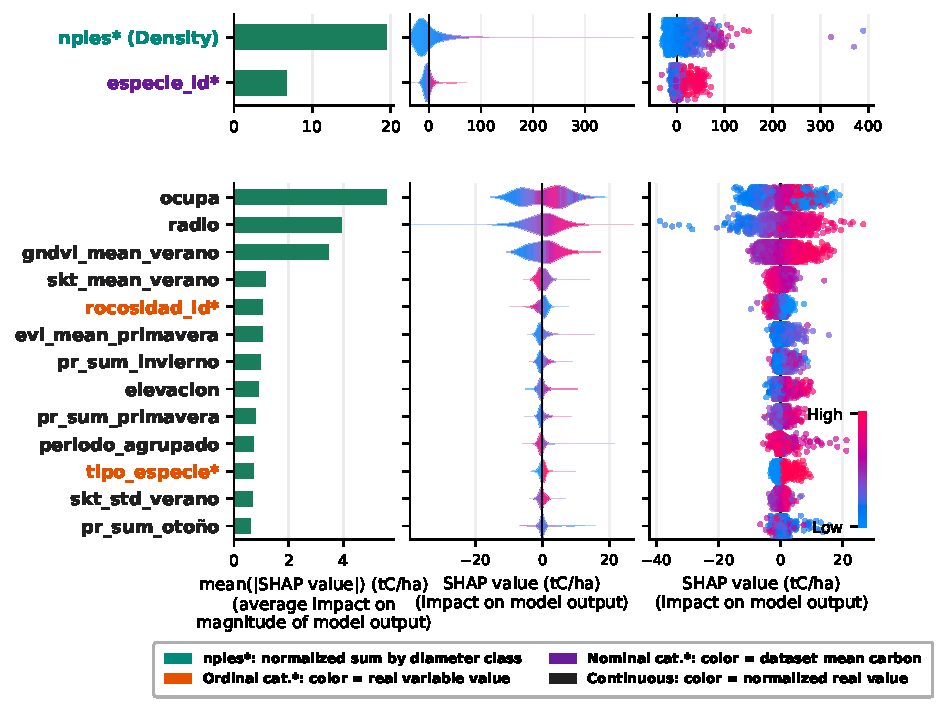
\includegraphics[width=\linewidth]{figuras/09_discusion/shap_summary_LightGBM_local_n2000_ifn2.pdf}
      \caption{SHAP analysis for the LightGBM model trained on IFN2 data with target variable \texttt{c4} (tC/ha).}
      \label{fig:SHAP_LightGBM_IFN2_c4}
\end{figure}

\begin{figure}
      \centering
      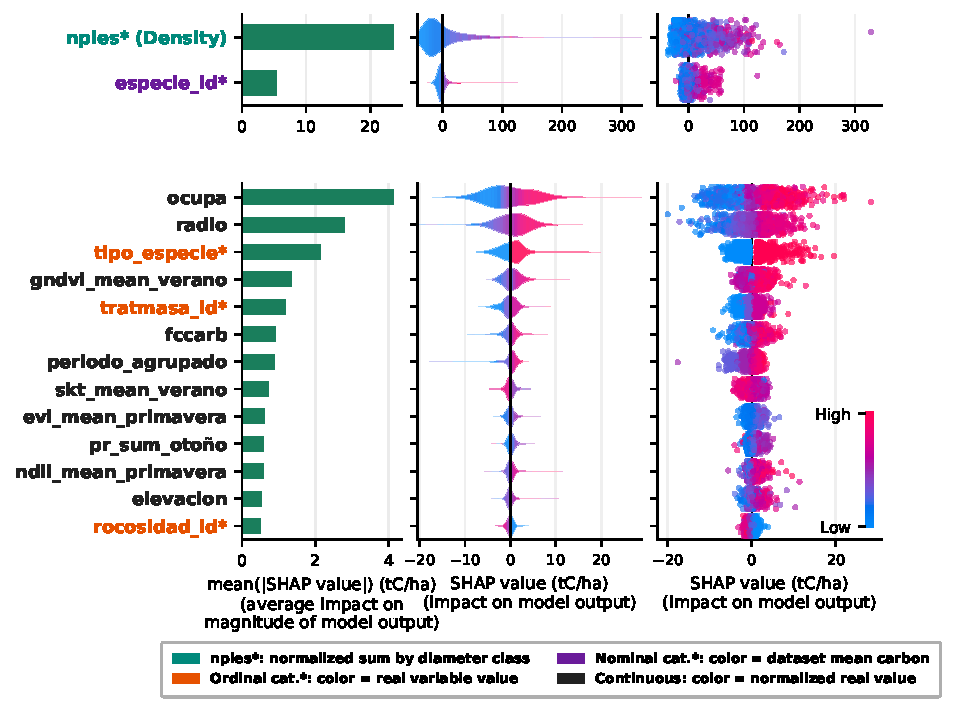
\includegraphics[width=\linewidth]{figuras/09_discusion/shap_summary_LightGBM_local_n2000_ifn3.pdf}
      \caption{SHAP analysis for the LightGBM model trained on IFN3 data with target variable \texttt{c4} (tC/ha).}
      \label{fig:SHAP_LightGBM_IFN3_c4}
\end{figure}

\begin{figure}
      \centering
      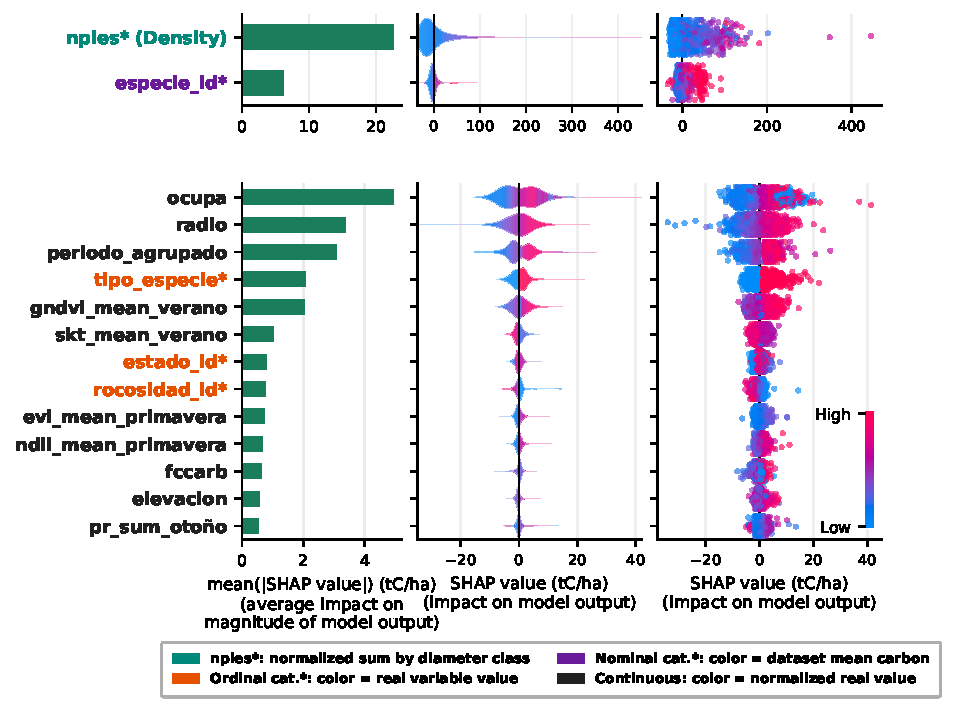
\includegraphics[width=\linewidth]{figuras/09_discusion/shap_summary_LightGBM_global_n2000_ifn23.pdf}
      \caption{SHAP analysis for the LightGBM model trained on IFN2 and IFN3 data with target variable \texttt{c4} (tC/ha).}
      \label{fig:SHAP_LightGBM_IFN2_3_c4}
\end{figure}


In Figures \ref{fig:SHAP_LightGBM_IFN2_c4}, \ref{fig:SHAP_LightGBM_IFN3_c4} and \ref{fig:SHAP_LightGBM_IFN2_3_c4} we see that the two most important variables are always \texttt{npies} and \texttt{especie\_id}, as we had seen in Table \ref{tab:shap_rank_abs}. The remaining variables change order depending on the case, but speaking of the whole set, the variables identified as important tend to be common across the three cases in the Figures. It should be noted that, although the positions of the variables do not exactly match between the case of the model trained solely with IFN2 data (Figure \ref{fig:SHAP_LightGBM_IFN2_c4}) and the model trained with IFN2 and IFN3 data (Figure \ref{fig:SHAP_LightGBM_IFN2_3_c4}), the variables present in the top $15$ shown are practically the same in total (except for \texttt{tratmasa\_id}) and \texttt{estado\_id} which are swapped. Variables exclusive to IFN3, such as \texttt{tratmasa\_id}, also appear, indicating that these new variables incorporated into successive inventories provide useful information for the study of forests, and specifically for studying carbon capture.

Looking at the values in Figures \ref{fig:SHAP_LightGBM_IFN2_c4}, \ref{fig:SHAP_LightGBM_IFN3_c4} and \ref{fig:SHAP_LightGBM_IFN2_3_c4} we can highlight some interesting results that support the idea that the model has correctly incorporated the information:
\begin{itemize}
      \item Looking at the variable \texttt{npies}, we observe that a higher number of initial trees corresponds to a higher SHAP value, i.e., more carbon.
      \item As stated earlier, for the variable \texttt{gndvi\_mean\_verano} a higher SHAP index is obtained for cases where its value is also higher. This is logical, since the GNDVI index measures photosynthetic activity. A higher value of this index corresponds to a greater presence of active vegetation, and therefore greater carbon capture.
      \item The variable \texttt{periodo\_agrupado} indicates the number of years between the measurement and the moment at which we wish to make the estimate, so it is expected that a higher value corresponds to a higher SHAP value, i.e., more carbon. This is what we find for the IFN3 case (Figure \ref{fig:SHAP_LightGBM_IFN3_c4}) and IFN2 and 3 (Figure \ref{fig:SHAP_LightGBM_IFN2_3_c4}). Curiously, for the IFN2 case (Figure \ref{fig:SHAP_LightGBM_IFN2_c4}) this relationship is less clear, which also coincides with the SHAP model assigning it relatively lower importance.
      \item The variable \texttt{tipo\_especie} has a very clear distinction in all cases. This is a binary variable in which value $0$ corresponds to conifers and value $1$ corresponds to broadleaves. According to the analysis, broadleaf species obtain on average a higher SHAP index, i.e., a greater amount of carbon associated with them. This is consistent with the literature, and specifically with studies carried out using the Spanish National Forest Inventory, which quantify the mean carbon \textit{stock} in broadleaf stands at $48.5 \pm 0.3$~Mg/ha compared to $41.8 \pm 0.2$~Mg/ha in conifers for mainland Spain \cite{vayreda2012carbon}.

      For further detail, Figure \ref{fig:SHAP_species_LightGBM_global} presents a breakdown of the SHAP index by species for the LightGBM model trained on data from both inventories and with \texttt{c4} as the target variable. It can be observed that broadleaves occupy almost all the positions in which carbon increases, with \textit{Eucalyptus globulus} as the first species, a species that has been causing controversy in northern Spain for years due to its possible characterisation as an invasive species \cite{miteco2017eucalyptus,greenpeace2025eucalipto}. However, it should be noted that this result reflects the biomass inventoried in the IFN, and does not imply that eucalyptus is the most appropriate option from a sustainable forest management perspective, given its high water consumption, its association with a higher fire risk, the loss of biodiversity it can cause, the difficulty of eradication, or the danger associated with the involuntary introduction of associated species, such as insects or fungi, displacing other native species \cite{miteco2017eucalyptus, cordero1999gonipterus, diez2005mycorrhizal}.
\end{itemize}

\begin{figure}
      \centering
      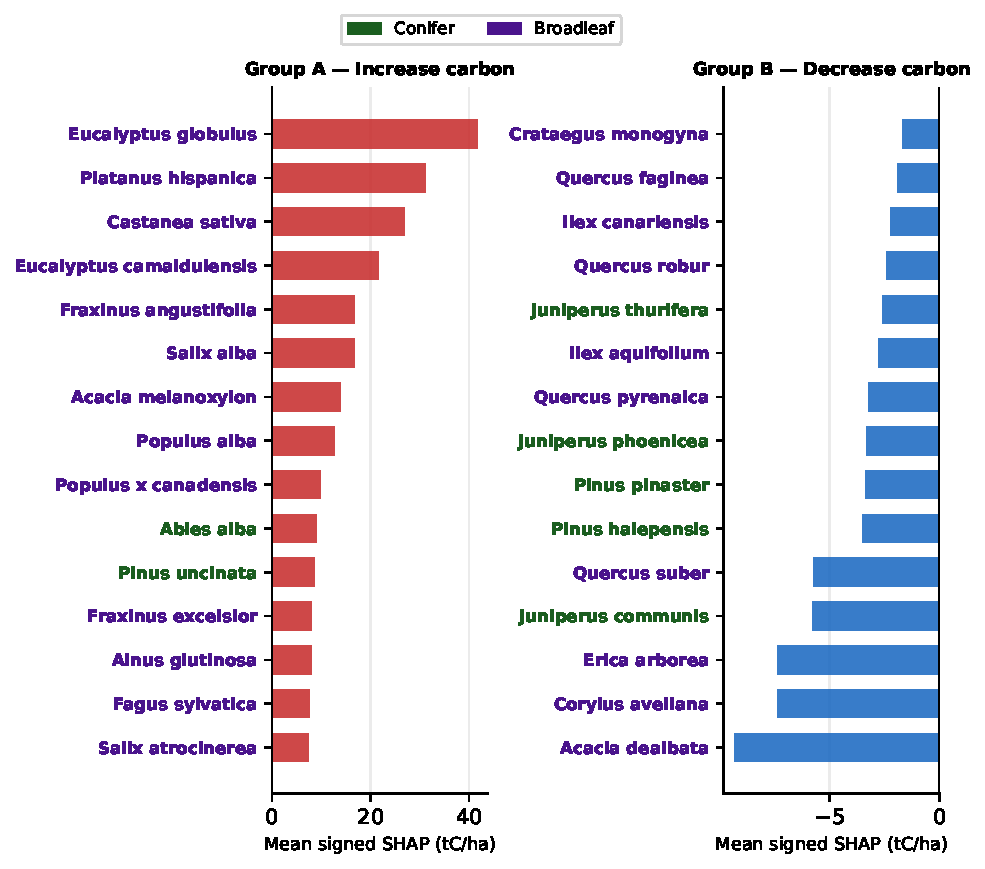
\includegraphics[width=\linewidth]{figuras/09_discusion/species_LightGBM_global.pdf}
      \caption{SHAP analysis for the LightGBM model trained on IFN2 and IFN3 data with target variable \texttt{c4} (tC/ha), focusing on species. A distinction is made between conifer and broadleaf.}
      \label{fig:SHAP_species_LightGBM_global}
\end{figure}

In summary, SHAP analysis not only allows identifying which variables are most relevant for carbon prediction and quantifying their relative importance, but also constitutes an ecological validation tool for the model. The results obtained are consistent with knowledge available in the literature: variables such as tree density, photosynthetic activity, species type or time elapsed between inventories show the expected direction in their SHAP values, indicating that the model has correctly incorporated the input information and that its predictions respond to real ecological processes.



% [Texto de ejemplo. Las figuras enlazadas son reales. El resto están en el repositorio de los modelos. Daltaría comentar el resto de casos.]

% \begin{figure}
%       \centering
%       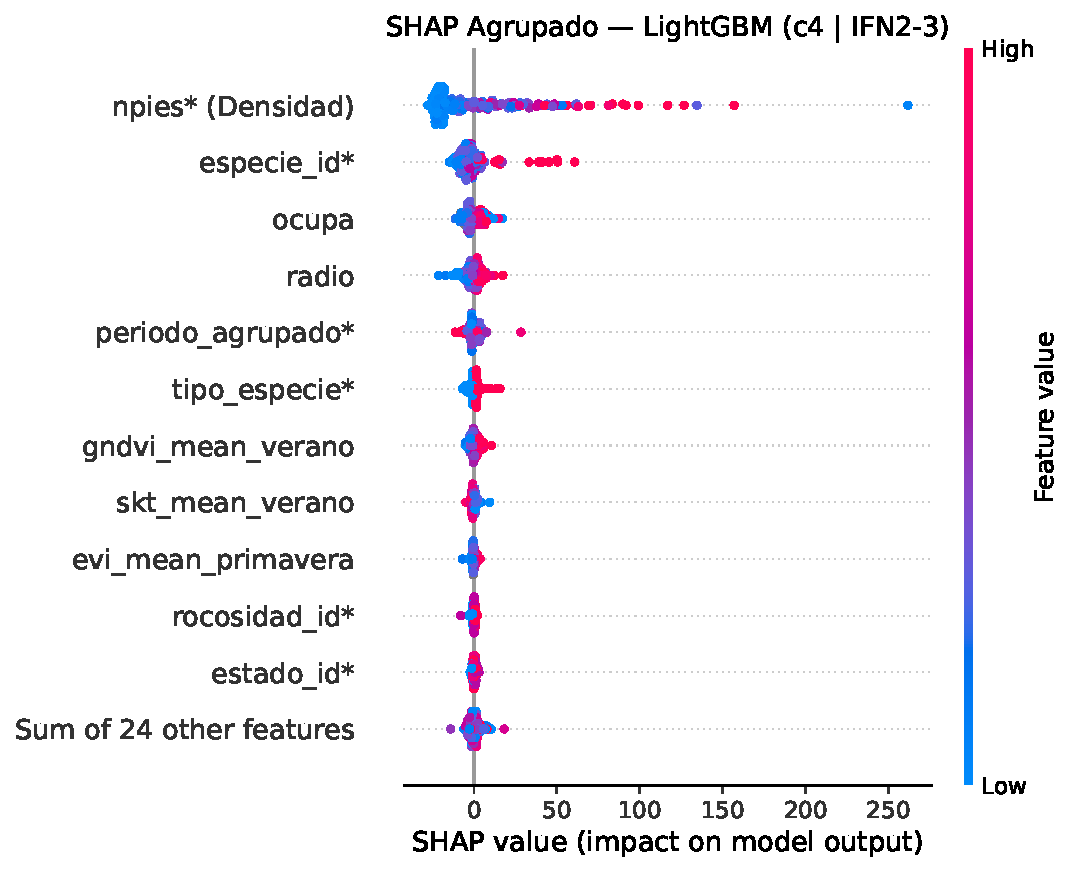
\includegraphics[width=\linewidth]{figuras/09_discusion/beeswarm_grouped_LightGBM.pdf}
%       \caption{Bee swarm plot of LightGBM for variable \texttt{carbono\_bruto4}.}
%       \label{fig:beeswarm_grouped_LightGBM}
% \end{figure}

% \begin{figure}
%       \centering
%       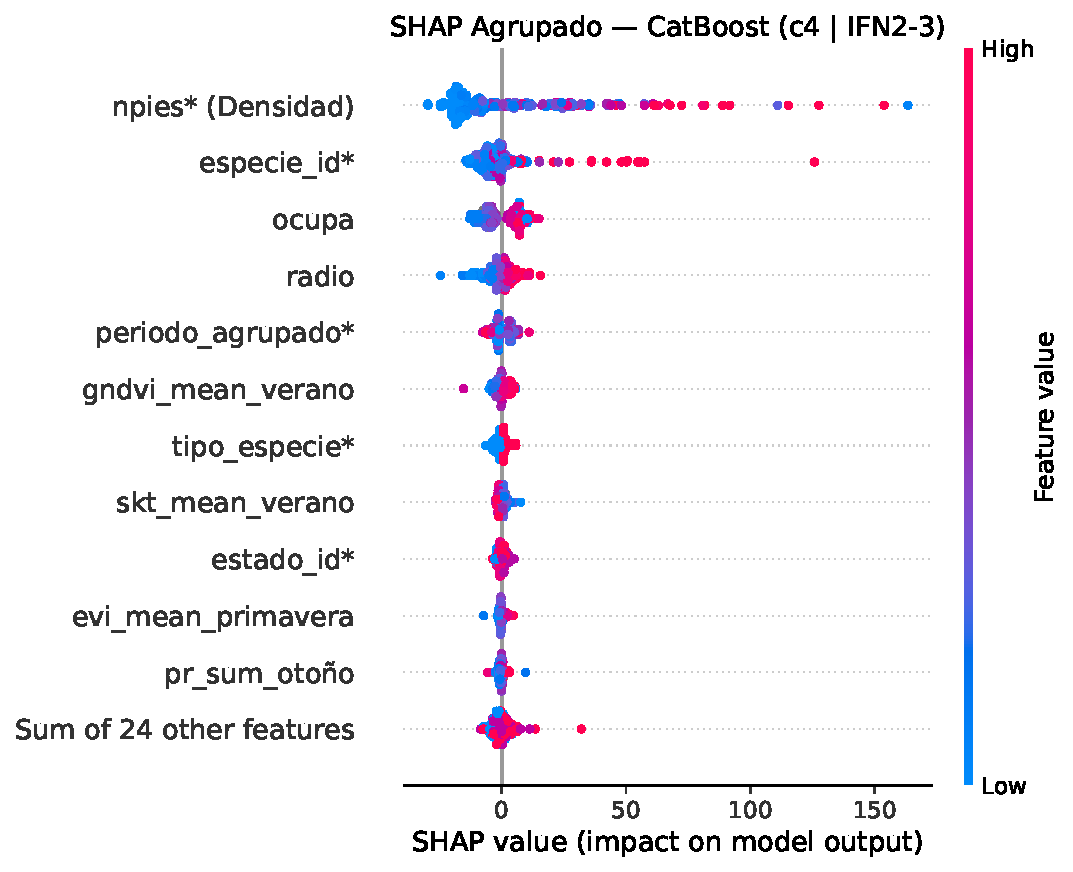
\includegraphics[width=\linewidth]{figuras/09_discusion/beeswarm_grouped_CatBoost.pdf}
%       \caption{Bee swarm plot of CatBoost for variable \texttt{carbono\_bruto4}.}
%       \label{fig:beeswarm_grouped_CatBoost}
% \end{figure}

\vspace{1cm}
\hrule
\vspace{1cm}

% !TEX root = ../main_final_en.tex
\section{Conclusions}
\label{sec:conclusiones}

The main objective of this work is the development of artificial intelligence models capable of predicting the carbon that a forest plot will capture over a given time horizon, based on structural, edaphic, climatic and spectral information collected in the National Forest Inventories and auxiliary data sources. The results obtained allow us to affirm that this objective has been satisfactorily achieved.

\subsection*{Feature selection and preprocessing}

The manual feature selection process (Section~\ref{sec:seleccion_variables}) allowed reducing an initial set of 445 candidate predictors to a compact subset of 44 variables, maintaining a balanced representation of all relevant ecological domains: stand structure, species composition, edaphic properties, terrain, climatology and spectral vegetation indices. This reduction not only facilitated the training of more efficient models, but also guaranteed the ecological interpretability of the selected predictors.

\subsection*{Model performance}

Models trained with IFN3 data as explanatory variables generally achieve the best metrics (see Table \ref{tab:top3_modelos}). This is explained by the higher quality, methodological homogeneity and richness of variables collected in this inventory compared to the IFN2.

Regarding the target variable, the prediction of carbon in absolute tonnes (\texttt{carbono\_bruto4}) is systematically more accurate in terms of global metrics than the prediction of carbon per unit area (\texttt{c4}, tC/ha), as can be seen by comparing Table \ref{tab:top3_modelos}. However, the decile analysis (Figures~\ref{fig:SMAPE_RMSE_deciles_c4_carbono_bruto4} and~\ref{fig:distribucion_carbono_bruto4_combinado}) reveals that for instances with very low carbon values (early biomass), relative errors (SMAPE) are high for both variables regardless of the model used. Models offer their best results in the intermediate-to-high biomass range, where the balance between data quantity, intrinsic variability and the magnitude of the target variable is most favourable.

The analysis of the \texttt{periodo} variable (Figures~\ref{fig:LightGBM_rmse_y_pct_rmse_cuantiles}, \ref{fig:Stack5_MLP_rmse_y_pct_rmse_cuantiles}, \ref{fig:CatBoost_combined} and~\ref{fig:Stack5_MLP_combined_rmse_y_pct_rmse_cuantiles}) shows that error grows with the prediction time horizon, especially when training data come from the IFN2 (periods exceeding 17 years). Nevertheless, median errors (quantile 50) remain relatively stable across all periods, indicating that the models correctly assimilate the average behaviour of forest growth even for long horizons. Extreme errors (quantile 90) are the most sensitive to data quality and temporal distance.

The sensitivity analysis on representative scenarios (Figures~\ref{fig:sensibilidad_escenarios} and~\ref{fig:sensibilidad_escenarios_carbono_bruto4}) confirms that the models qualitatively correctly capture the growth dynamics: the general trend is upward with the period, and the models reproduce the effects of the inventory changes (from IFN2 to IFN3) observed in the real data.

\subsection*{Global versus local models}

The comparison between ``global'' models (trained on IFN2 and IFN3 jointly) and ``local'' models (trained on a single inventory), shown in Figures~\ref{fig:comparativa_mejores}--\ref{fig:disc_sub4} and in Table~\ref{tab:top3_modelos}, reveals differentiated behaviour depending on the validation inventory. For IFN3, local models outperform global ones, since the inclusion of IFN2 data introduces heterogeneity that penalises prediction on higher-quality data. For IFN2, in contrast, global models are superior, as they benefit from the additional patterns learned with the IFN3 data. This result underscores that the choice of training set must be adapted to the time horizon and the target inventory.

\subsection*{\textit{Stacking} models}

The incorporation of stacking schemes produces systematic but modest improvements over the best base models (see Table~\ref{tab:top3_modelos}). The stacking ensemble with configuration 5 and MLP meta-model is consistently the one that achieves the best metrics for both \texttt{c4} and \texttt{carbono\_bruto4}. The fact that the improvement is systematic in all cases rules out it being a statistical artefact, but its limited magnitude raises the question of whether the additional complexity of stacking is justified compared to using the best individual model in a hypothetical production system. Gradient boosting-based algorithms, especially CatBoost and LightGBM, offer the best performance as base models in all evaluated scenarios.

\subsection*{Interpretability}

The SHAP value analysis (Section~\ref{sec:interpretabilidad_shap}, Table~\ref{tab:shap_rank_abs}) confirms that structural stand variables ---tree density (\texttt{npies}), species (\texttt{especie_id}), canopy cover fraction (\texttt{ocupa}) and plot radius (\texttt{radio})--- are the dominant predictors regardless of the source inventory or target variable considered. Among the auxiliary variables, the summer GNDVI index (\texttt{gndvi_mean_verano}) emerges as the most informative spectral predictor, consistent with its capacity to estimate photosynthetic activity without saturation in dense canopies. The direction of SHAP values is in all cases consistent with available ecological knowledge: higher tree density, greater photosynthetic activity and longer time horizons lead to higher predicted carbon; broadleaves systematically outperform conifers, in line with the mean \textit{stocks} reported in the literature for mainland Spain \citep{vayreda2012carbon}. This indicates that the models are not only numerically accurate, but have learned relationships with genuine ecological meaning, which reinforces their interpretability and confidence for a possible practical application.

\subsection*{Comparison with the literature}

In similar works, such as that of \citet{fasihi2024assessing} for northern Italy, forest carbon values are predicted from remote sensing observations without the use of field-measured in situ data. Although the context is different ---they predict the carbon present at the time of measurement, without temporal projection--- the errors they report are notably higher than those obtained in this work, especially in the shortest prediction range (around 5 years), which is the most comparable. This highlights the added value of incorporating structural field information (IFN) compared to approaches based exclusively on remote sensing.

\subsection*{Limitations}

The main limitation of the study lies in the heterogeneity and irregularity of the available data. The distribution of instances as a function of the \texttt{periodo} variable is very unequal: some years have thousands of samples while others have barely a few dozen. This irregularity, inherent to the nature of the Forest Inventories (conducted over different time periods and with methodologies that evolve between iterations), limits the model's capacity for certain time horizons, particularly in the range of years with fewer data and where the main source is the IFN2. Despite this, the models demonstrate reasonable generalisation capacity even under these conditions.

\subsection*{Future work and applicability}

For a possible production application as a decision-support system for carbon project recommendations, it would be necessary to evaluate the extent to which IFN plots are representative of forest plantations intended for carbon credits, which may differ in density, management and composition. A natural extension of the model would be to incorporate LiDAR data, whose capacity to characterise the three-dimensional structure of the forest canopy has been shown in other studies to significantly improve biomass and carbon predictions \citep{nyakudanga_treemes}. Likewise, adapting the model to other geographical contexts or integrating it with IFN4 data as the target variable constitute promising lines of future work.

% !TEX root = ../main_final_en.tex
% sections/10_agradecimientos.tex
\section*{Acknowledgements} % Use \section* so this section is not numbered

Research funded by grant \textbf{TSI-100933-2023-1} from the \textbf{Call for University-Business Chairs (ENIA Chairs 2022), Ministry of Digital Transformation and Civil Service of Spain}, and the \textbf{EU Recovery and Resilience Plan} (\textit{NextGenerationEU/PRTR}).


\clearpage
\bibliographystyle{model1-num-names}
\bibliography{referencias}

\appendix
\onecolumn
\input{sections_en/12_annex_results_global}

\end{document}
